%!TEX root = ../thesis_a4.tex

\chapter{Data Pre-processing}
\label{chap:data_preprocessing}


\section{Introduction}
\label{sec:data_preprocessing_intro}

In this chapter we describe the pre-processing steps followed to obtain different data representations from audio music signals. These compact and musically meaningful representations derived from raw audio data are used as input to different methods described later in this dissertation. Since a number these methods start by performing the same data transformation, we consolidate and present these common pre-processing blocks in the same chapter. This chapter is based on work already presented in XXXX. In the subsequent sections we describe the process followed for identifying the tonic of the lead artist XXXX, for estimating the pitch of the predominant melodic source (typically the lead artist) and transforming it from Hertz to Cents scale, and detecting \gls{nyas} segments in the melodies of \gls{iam}.

Along with the description of these processing blocks we also provide sufficient implementation details and the parameter values used in the experiments. For certain experiments the parameter settings might differ from the one presented in this chapter. In such cases the precise value of the parameters is given in the description of the respective method.

\TODO{Do we need to provide the motivation or need for data pre-processing or this is obvious?}

%In this thesis we follow a data-driven methodology to devise computational models for melodic analysis of \gls{iam}.  In the scope of this work data primarily corresponds to a collection of annotated audio music recordings. Before we start to model the human perception and cognition functions associated with a task, we transform the raw audio data and derive a higher level representation. Such an abstracted representation compactly captures the essential musical characteristics that XXXX. 
%
%In this chapter we present different representations of the data used across the experiments in this thesis and describe the procedure to extract them from the raw audio signals. Since several experiments share the step of data transformation, it is summarized in this chapter at once. 


%Thoughts
%\begin{itemize}
%	\item What do we mean by data here, what kind of data are we using. Data-> input that we feed to our algorithms. In the scope of this thesis its primarily the audio data + small amount of metadata. The pre-processing is only for the audio data. 
%	\item What do we mean by data pre-proessing. why is it called pre-processing. Audio data is a very low level physical data, before we can use it or make sense out of it we have to abstract it. We have to transform the data and extract a representation of the concept that we are working on. This is how most of the algorithms discussed in this paper function. Typically these processing involve converting audio data to a perceptual representation. On which further cognitive models are applied to extract high level information which has a musical interpretation or is musically meaningful. 
%	\item Why do we have to do pre-processing, what is the reason/motivation
%	\item What kind of pre-processing do we do. 
%	\item Why have we written this at the beginning at one place, its been used in almost every module in the paper
%	\item How is this chapter organized. 
%\end{itemize}

\section{Tonic Identification: Approaches and Comparative Evaluation}
\label{sec:data_preprocessing_tonic_identification}

The tonic pitch of a lead artist is the base frequency that serves as a reference and foundation for melodic integration throughout the performance (Section\TODO{secref}). All the tones in the musical progression are always in reference and related to the tonic pitch. The accompanying instruments such as tabl\={a} and violin are tuned to the tonic of the lead performer. In a performance of \gls{iam} tonic pitch in majority of the cases corresponds to the \textit{Sa} \gls{svara} of the \gls{raga} (the exceptions are the madhyam \gls{shruti} cases in Carnatic music). Other \glspl{svara} used in the performance derive their meaning and purpose in relation to the \textit{Sa} \gls{svara} and the tonal context established by the particular \gls{raga}~\citep{Danielou2010}. Identification of tonic pitch is therefore a crucial first step for tonal analysis of \gls{iam}. In Particular, for a meaningful comparison of melodies across artists, it is important that the melodic representation is normalized by the tonic of the lead artist. Identification of the tonic pitch of the lead artist in a recording is therefore typically a pre-processing step in most of the melodic analyses of \gls{iam}. 

There exist a number of approaches for identifying tonic pitch in an audio recording of \gls{iam}~\citep{salamon2012multipitch,gulati2012two,bellur2012knowledge,ranjani2011carnatic,Sengupta2005b}\TODO{{add parags method and then say why it wasn't considered for the evaluation}}. Our previous works on tonic identification show promising results with accuracy close to 90\%~\citep{salamon2012multipitch,gulati2012two}. However, it might be misleading to draw a consensus on the best performing method based on just the reported accuracy. This is because these approaches are evaluated using different datasets with varied musical characteristics and under different experimental setup. Therefore, to select the most promising approach we perform a thorough comparative evaluation on the same set of datasets and under the same experimental setup~\citep{Gulati2014Tonic}. The evaluation is performed using a number of scalable datasets with varied musical and acoustical characteristics that are representative of real-world collections of \gls{iam}. In the subsequent sections we describe the comparative evaluation, which is based on our earlier work presented in~\cite{Gulati2014Tonic}. In order for this dissertation to be self-contained, we start by providing a brief description of the methods we evaluated~(\secref{sec:pre_processing_tonic_identification_existing_approaches}). We then describe the experimental setup and the datasets used for the comparative evaluation~(\secref{sec:pre_processing_experimental_setup}). We present the results of the comparative evaluation and highlight the strengths and limitations of the methods on different type of music material~(\secref{sec:pre_processing_tonic_identification_results}). Finally, we explain a heuristic-based approach to correct common mistakes in tonic identification in a collection of \gls{iam} by exploiting associated metadata of a recording. 


\subsection{Existing Approaches}
\label{sec:pre_processing_tonic_identification_existing_approaches}

As mentioned, there have been various efforts to automatically identify the tonic pitch of the
lead artist in a performance of Indian art music~\citep{salamon2012multipitch,gulati2012two,bellur2012knowledge,ranjani2011carnatic,Sengupta2005b}.
These approaches mainly differ in terms of the musical cues that they utilize to
identify the tonic, the amount of input audio data used to perform this task and the type
of music material they are devised for (Hindustani or Carnatic, vocal or
instrumental, etc.). Despite the differences, all these approaches can be divided
into three main processing blocks, as shown in~\figref{fig:tonic_identification_general_block_diagram}. The only exception to this schema is the approach proposed by~\citep{Sengupta2005b}.

\begin{figure}
	\begin{center}
		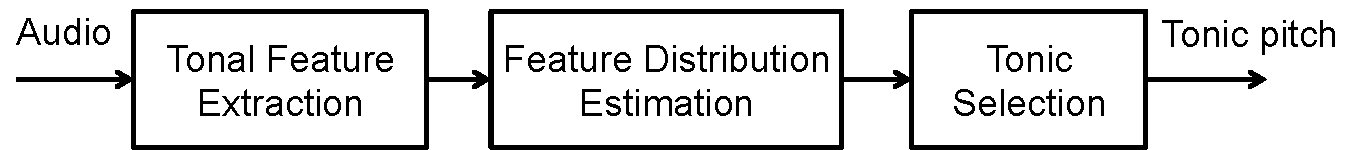
\includegraphics[width=\figSizeNinety]{ch05_preprocessing/figures/tonic_identification_block_diagram.pdf}
	\end{center}
	\caption[General block diagram of the processing steps used by tonic identification
	approaches.]{General block diagram of the processing steps used by tonic identification
		approaches.}
	\label{fig:tonic_identification_general_block_diagram}
\end{figure}


In all the aforementioned approaches, the three main processing blocks are the following: feature
extraction, feature distribution estimation and tonic selection. Since the task
of tonic identification involves an analysis of the tonal content of the audio
signal, the features extracted in the first block are always pitch related. In
the second block, an estimate of the distribution of these features is obtained
using either Parzen window based density estimation or by constructing a
histogram. The feature distribution is then used in the third block to identify
the tonic. The peaks of the distribution correspond to the most salient pitch
values used in the performance (usually the \glspl{svara} of the \gls{raga}), one of which
corresponds to the tonic pitch. As the most salient peak in the distribution is
not guaranteed to be the tonic, various techniques are applied to select the peak that corresponds to the tonic.



{\renewcommand{\arraystretch}{1.5}
	\begin{sidewaystable} 
		\begin{centering}
			\begin{tabular}{ c c c c }
\tabletop			
			Method 	&	Features	&	Feature Distribution	&	Tonic Selection \\
\tablemid			
			\acrshort{tonicid_sengupta} \citep{Sengupta2005b}	&	Pitch \citep{AKDatta_1996} & N/A & Error minimization\\
			
			\acrshort{tonicid_ranjani_1}/\acrshort{tonicid_ranjani_2} \citep{ranjani2011carnatic}	&	Pitch \citep{BoersmaPaul2001} & Parzen-window-based \acrshort{pde}  & GMM fitting\\
			
			\acrshort{tonicid_justin} \citep{salamon2012multipitch} & Multi-pitch salience \citep{Salamon2011} & Multi-pitch histogram & Decision tree\\

			\acrshort{tonicid_sankalp} \citep{gulati2012two}	& Multi-pitch salience  \citep{Salamon2011} & Multi-pitch histogram & Decision tree\\

			&	Predominant melody \citep{Salamon2012} & Pitch histogram & Decision tree\\

			\acrshort{tonicid_ashwin_1} \citep{bellur2012knowledge}	&	Pitch \citep{DeCheveigne2002}	&  \acrshort{gd} histogram & Highest peak\\

			\acrshort{tonicid_ashwin_2} \citep{bellur2012knowledge}	&	Pitch \citep{DeCheveigne2002}	& 	GD histogram	&
			Template matching\\

			\acrshort{tonicid_ashwin_2} \citep{bellur2012knowledge}	&	Pitch \citep{DeCheveigne2002}	& 	GD histogram
			& Highest peak\\
			
			\acrshort{tonicid_chordia}	& 	& 	& \\			

\tablebot			
			\end{tabular}

			\caption[Summary of existing tonic identification approaches.]{Summary of existing tonic identification approaches.}
			\label{tab:pre_processing_tonic_identification_summary_methods}
			\par \end{centering}	
	\end{sidewaystable}


In \tabref{tab:pre_processing_tonic_identification_summary_methods} we provide a summary of the existing methods for tonic identification. The common processing blocks and the main differences between them become evident from this table. A detailed review of these methods in terms of the three processing stages as shown in \figref{fig:tonic_identification_general_block_diagram} is done in~\cite{Gulati2014Tonic}. For a more detailed description of these methods we refer to their respective publications listed in Table \tabref{tab:pre_processing_tonic_identification_summary_methods}. 

\TODO{description of the methods?}

\subsection{Comparative Evaluation Setup}
\label{sec:pre_processing_experimental_setup}

In order to select the best method for tonic identification in audio collections of \gls{iam} we perform a comparative evaluation. We evaluate seven of the nine tonic identification methods listed in \tabref{tab:pre_processing_tonic_identification_summary_methods} using the same set of datasets. The methods chosen for evaluation are
denoted by \acrshort{tonicid_justin}~\citep{salamon2012multipitch}, \acrshort{tonicid_sankalp}~\citep{gulati2012two}, \acrshort{tonicid_ranjani_1} and \acrshort{tonicid_ranjani_2}~\citep{ranjani2011carnatic}, \acrshort{tonicid_ashwin_1}, \acrshort{tonicid_ashwin_2} and \acrshort{tonicid_ashwin_3}~\citep{bellur2012knowledge}. Note that \acrshort{tonicid_sengupta}~\citep{Sengupta2005b} was not available for
evaluation and \acrshort{tonicid_chordia} was not available when the experiments were conducted. 

Each of the method mentioned above is evaluated using six different datasets, denoted \acrshort{tds_cm1}, \acrshort{tds_cm2}, \acrshort{tds_cm3}, \acrshort{tds_iitm1}, \acrshort{tds_iitm2} and \acrshort{tds_iisc}. A detailed description of these datasets in terms the musical material and the audio quality is given in~\secref{sec:corpus_tonic_datasets}. A quick summary of the datasets can be obtained from~\tabref{tab:tonic_datasets}. The diversities present in real-world music collections of \gls{iam} in terms of the varied musical and acoustical characteristics are well captured in these six datasets. Note that \acrshort{tonicid_ashwin_1} requires several excerpts from the same concert in order to compute the segmented \gls{gd} histogram, and this kind of data (and metadata) is only available for \acrshort{tds_iitm1} dataset. Hence, \acrshort{tonicid_ashwin_1} is only evaluated using \acrshort{tds_iitm1} dataset.

For vocal performances we evaluate the accuracy of correctly identifying the tonic pitch, whereas for instrumental music we evaluate the accuracy of estimating the tonic pitch-class only (i.e.~the identified tonic pitch is allowed to be in any octave). This is because whilst for vocal music the concept of the tonic pitch being in a specific octave is clearly defined (because it is restricted by the pitch range of the singer), this notion is not as clear for instrumental music. For vocal performances, the tonic identified by a method is considered correct if it is within 50 cents of the ground truth annotation. For instrumental music, a method's estimate is considered correct if it is within 50 cents of the correct tonic pitch-class.

Classification-based approaches, which require training (\acrshort{tonicid_justin} and \acrshort{tonicid_sankalp}) are evaluated by performing 10-fold cross-validation on every dataset, repeating
every experiment 10 times and reporting the mean accuracy over the 10 repetitions. All parameters are kept fixed for all methods across all datasets. Since tonic pitch range for male and female singers, and for instrumental music is different, editorial metadata regarding the gender of the singer and the type of music excerpt (vocal or instrumental) can be used to improve the accuracy of tonic identification. We therefore perform two sets of experiments, one with only using the audio excerpts, and the other in which the methods are also given information about the gender of the singer and the type of excerpt (vocal or instrumental). 

\subsection{Results and Discussion}
\label{sec:pre_processing_tonic_identification_results}

In this section we present the results of the comparative evaluation. We compare the performance of different tonic identification approaches, highlight their shortcomings and discuss various types of errors made by them. The section is divided into three parts: in ~\secref{sec:pre_processing_tonic_id_results_only_audio_data} we present the results obtained when only the audio data is used and no additional metadata is provided to the methods. Subsequently, we report the performance accuracy
obtained when information regarding the gender of the singer (male or female) and performance type (instrumental or vocal) is provided to the methods in addition to the audio data (\secref{Results obtained using metadata together with the audio}). Finally in \secref{Error Analysis} we present an analysis of the most common errors made by the methods and make some general observations regarding their performances.

\subsubsection{Results Obtained Using Only Audio Data}
\label{sec:pre_processing_tonic_id_results_only_audio_data}

In Table~\ref{tab:tonic_identification_accuracy_without_gender_info} we summarize the
identification accuracies (in percentage) for tonic pitch (TP) and tonic
pitch-class (TPC) obtained by seven methods on six datasets, using
only audio data.

{\renewcommand{\arraystretch}{1.4}
\setlength{\tabcolsep}{10pt}
\begin{sidewaystable}
	\centering
	\begin{tabular}{ c | c  c : c  c : c  c : c  c : c  c : c  c }
\tabletop
		\multirow{2}{*}{Methods}  & \multicolumn{2}{ c: }{\acrshort{tds_cm1}} & \multicolumn{2}{ c: }{\acrshort{tds_cm2}} & \multicolumn{2}{ c: }{\acrshort{tds_cm3}}  &    \multicolumn{2}{ c: }{\acrshort{tds_iisc}}  &  \multicolumn{2}{ c: }{\acrshort{tds_iitm1}}  & \multicolumn{2}{ c}{\acrshort{tds_iitm2}} \\
		\cline{2-13}
		{} & TP & TPC    & TP & TPC & TP & TPC & TP & TPC
		& TP & TPC & TP & TPC   \\
\tablemid
		\acrshort{tonicid_justin} & - & 88.9 & 87.4 & 90.1 & \textbf{88.4} & \textbf{91} & 75.6 & 77.5 & 	89.5 & \textbf{97.4} & 90.8 & \textbf{94.1}\\

		\acrshort{tonicid_sankalp} & - & \textbf{92.2} & \textbf{87.8} & \textbf{90.9} & 87.7 & 90.5 &
		79.8 & \textbf{85.3} & \textbf{97.4} & \textbf{97.4} & \textbf{93.6}
		& 93.6  \\
		
		\hdashline
		
		\acrshort{tonicid_ranjani_1} & - & 81.4 & 69.6 & 84.9 & 73.2 & 90.8 & 81.8 & 83.6 & 92.1 & \textbf{97.4} &
		80.2 & 86.9  \\
		
		\acrshort{tonicid_ranjani_2} & - & 63.2 & 65.7 & 78.2 & 68.5 & 83.5 & \textbf{83.6} & 83.6 & 94.7 &
		\textbf{97.4} & 83.8 & 88.8\\
		
		\acrshort{tonicid_ashwin_1} & - & - & - & - & - & - & - & - & 89.5 & 89.5 & - & - \\
		
		\acrshort{tonicid_ashwin_2} & - & 88.9 & 74.5 & 82.9 & 78.5 & 83.4 & 72.7 & 76.4 & 92.1 & 92.1 & 86.6   & 89.1 \\
		
		\acrshort{tonicid_ashwin_3} & - & 86 & 61.1 & 80.5 & 67.8 & 79.9 & 72.7 & 72.7 & 94.7 & 94.7 & 85  & 86.6 \\
\tablebot
	\end{tabular}
	\caption[Tonic identification accuracies of seven methods on six different datasets. These accuracies are when no metadata is used in addition to audio data.]{Accuracies for tonic pitch (TP \%) and tonic pitch-class (TPC \%) identification by seven methods on six different datasets using only audio data. The best accuracy obtained for each dataset is
	highlighted using bold text. The dashed horizontal line divides the methods based on supervised learning (\acrshort{tonicid_justin} and \acrshort{tonicid_sankalp}) and those based on expert knowledge (\acrshort{tonicid_ranjani_1}, \acrshort{tonicid_ranjani_2}, \acrshort{tonicid_ashwin_1}, \acrshort{tonicid_ashwin_2} and \acrshort{tonicid_ashwin_3}). TP column for \acrshort{tds_cm1} is marked as `-', because it consists of only instrumental excerpts for which we not evaluate tonic pitch accuracy.}
	\label{tab:tonic_identification_accuracy_without_gender_info}
\end{sidewaystable}

From \tabref{tab:tonic_identification_accuracy_without_gender_info} we see that most of the methods perform well on all datasets, and the accuracy of the best performing method on each dataset ranges from 84-97\%. We note that the identification accuracy obtained for instrumental music (\acrshort{tds_cm1}) by each method is comparable to the accuracy obtained for vocal music, meaning the approaches are equally suitable for vocal and instrumental music. The approaches based on multi-pitch analysis and classification (\acrshort{tonicid_justin} and \acrshort{tonicid_sankalp}) are more consistent and perform better across different datasets compared to the approaches based only on predominant pitch (with the exception of \acrshort{tds_iisc}, most likely due its poor recording quality). We see that the performance of both the multi-pitch based approaches is comparable. As could be expected, the simple maximum peak selection approach employed by \acrshort{tonicid_ashwin_1} and \acrshort{tonicid_ashwin_3} is too simplistic and the template matching approach employed in \acrshort{tonicid_ashwin_2} yields better results in most cases. 

\acrshort{tonicid_sankalp} obtains the best results for the instrumental dataset \acrshort{tds_cm1}, with \acrshort{tonicid_ashwin_2} and \acrshort{tonicid_justin} reporting comparable accuracies. For the \acrshort{tds_cm2} and \acrshort{tds_cm3} datasets, we see that the multi-pitch based approaches (\acrshort{tonicid_justin} and \acrshort{tonicid_sankalp}) obtain the best performance, whilst the predominant pitch based methods exhibit a considerable difference between the TP and TPC accuracies. This means that in many cases these approaches are able to identify the tonic pitch-class correctly but fail to identify the correct octave of the tonic pitch. In the case of \acrshort{tonicid_ranjani_1}, \acrshort{tonicid_ranjani_2}, \acrshort{tonicid_ashwin_2} and \acrshort{tonicid_ashwin_3}, this can be attributed primarily to the tonic selection procedure employed by these approaches. The group-delay processing used in \acrshort{tonicid_ashwin_2} and \acrshort{tonicid_ashwin_3}, and the estimators used in \acrshort{tonicid_ranjani_1} and \acrshort{tonicid_ranjani_2}, accentuate the peaks corresponding to all \glspl{svara} that have a low degree of pitch variance. This includes both the lower and higher octave \gls{shadja} and panchama in addition to the middle octave \gls{shadja} (the tonic pitch). Furthermore, the magnitude of peaks corresponding to \gls{shadja} in higher and lower octave is sometimes further accentuated by pitch halving and doubling errors produced by the pitch extraction algorithm. This makes identification of the correct tonic octave more difficult and as seen in Table~\ref{tab:tonic_identification_accuracy_without_gender_info}, results in a higher degree of octave errors.

When considering the results for the \acrshort{tds_iisc} dataset, we note that the performance drops for all methods. The main reason for this is the poor audio quality of the excerpts in this collection. The recordings are relatively old and noisy, and contain a humming sound in the background. This makes pitch
tracking very difficult. Furthermore, the drone sound in the recordings is very weak compared to the lead artist, which explains the drop in performance for the multi-pitch based approaches. If we consider performance for \acrshort{tds_iitm1} on the other hand, we see that all methods perform very well. This is because each excerpt in this dataset is a full concert, which includes many performances in different \glspl{raga}. Usually different set of \glspl{svara} are used in different performances, but with the same tonic pitch throughout the concert. As a result, the melody histogram contains a very high peak corresponding to the Sa \gls{svara}, making it considerably easier to identify the tonic pitch.

\begin{figure}
	\begin{center}
		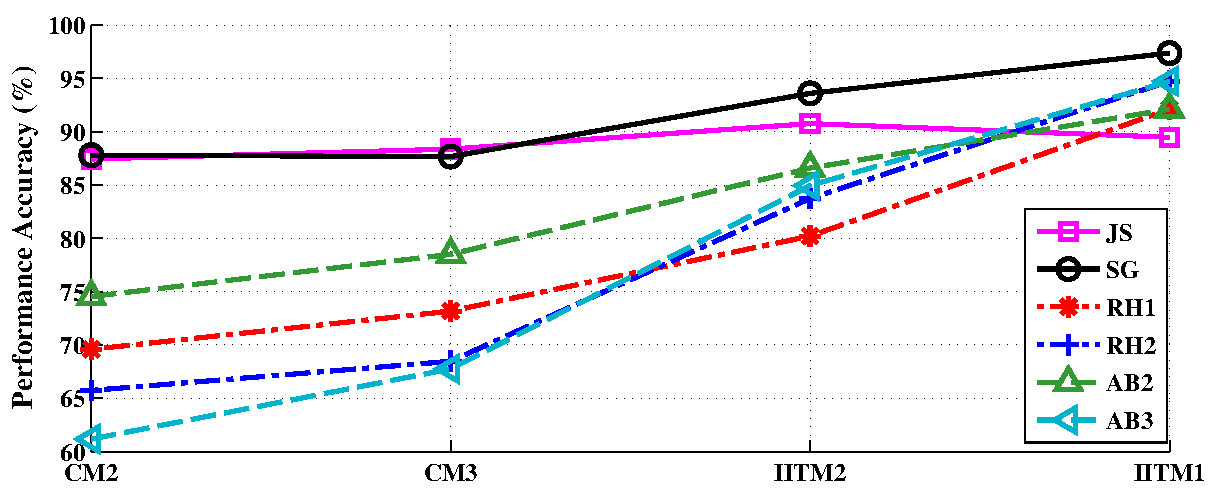
\includegraphics[width=\figSizeNinety]{ch05_preprocessing/figures/Accuracy_Length.pdf}
	\end{center}
	\caption{Accuracy (\%) of different methods on four datasets arranged
		by increasing order of mean duration.\TODO{Fix method and dataset names}}
	\label{fig:tonic_id_accuracy_vs_length}
\end{figure}


We now proceed to analyze the tonic identification accuracy as a function of the excerpt duration. As shown in~\tabref{tab:tonic_datasets}, different datasets contain audio excerpts of different lengths. In order to investigate a possible correlation between the accuracy of a method and the length of an audio
excerpt, in~\figref{fig:tonic_id_accuracy_vs_length} we plot the identification accuracies of the different methods for four of the six datasets ordered
by the mean duration of the excerpts: \acrshort{tds_cm2} (3 min), \acrshort{tds_cm3} (full song), \acrshort{tds_iitm2} (full song) and \acrshort{tds_iitm1} (full concert). \acrshort{tds_cm1} and \acrshort{tds_iisc} are excluded because the characteristics of these datasets are very different compared to the rest of the datasets (\acrshort{tds_cm1} contains only instrumental performances and \acrshort{tds_iisc} has poor quality audio). As could be expected, from~\figref{fig:tonic_id_accuracy_vs_length} we notice that practically for all methods there is an improvement in the performance as we increase the duration
of the excerpts. Interestingly, the improvement is very significant for the predominant pitch based methods (\acrshort{tonicid_ranjani_1}, \acrshort{tonicid_ranjani_2}, \acrshort{tonicid_ashwin_2} and \acrshort{tonicid_ashwin_3}) compared to the multi-pitch based methods (\acrshort{tonicid_justin} and \acrshort{tonicid_sankalp}). This implies that the latter approaches, which exploit the pitch information of the drone instrument, are more robust to the duration of audio data.

\begin{figure}
	\begin{center}
		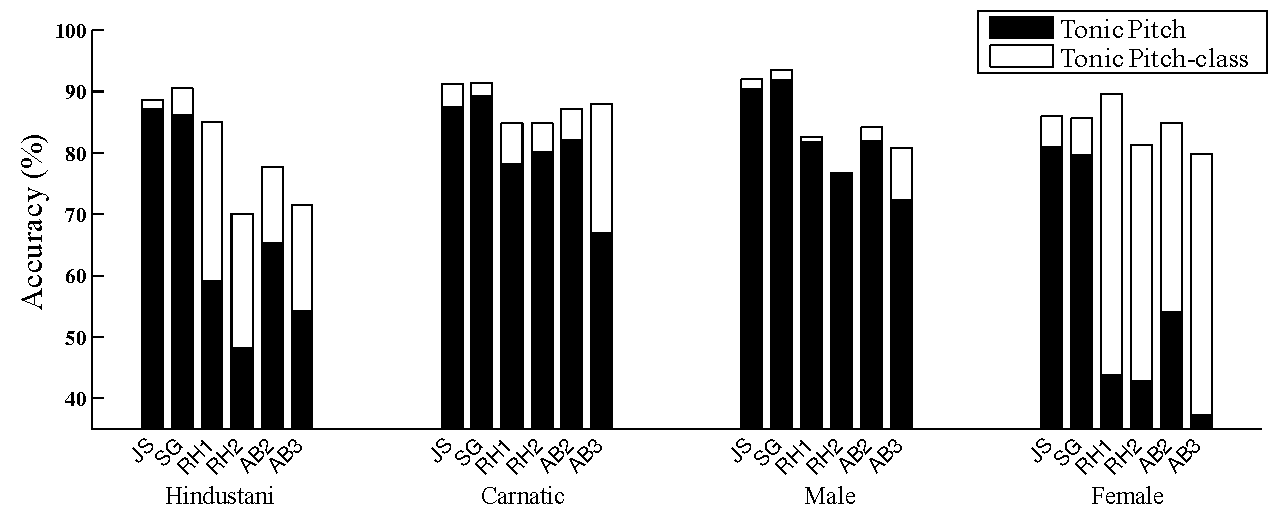
\includegraphics[width=\figSizeHundred]{ch05_preprocessing/figures/Category_Performance.pdf}
	\end{center}
	\caption{Accuracy (\%) as a function of different attributes
		(Hindustani, Carnatic, male, female).\TODO{Fix method and dataset names}}
	\label{fig:tonic_id_categorywise_performance}
\end{figure}

In addition to analyzing the performance accuracy for the whole dataset, we also examine the results as a function of different attributes of
the audio excerpts, namely music tradition (Hindustani or Carnatic) and the gender of the lead singer (male or female). For this analysis we use the \acrshort{tds_cm2} dataset, as it has the most balanced representation of excerpts from the different categories. In~\figref{fig:tonic_id_categorywise_performance} we show the accuracies obtained by the different methods as a function of the different attributes. We see that the performance of the multi-pitch based approaches (\acrshort{tonicid_justin} and \acrshort{tonicid_sankalp}) is relatively independent of the music tradition (Hindustani or Carnatic). On the other hand, for the predominant pitch based approaches there is a significant difference in performance for Hindustani and Carnatic music. They obtain considerably better results on Carnatic music. The most notable difference for these approaches is the increased amount of octave errors made for Hindustani music compared to Carnatic music (deduced from the difference seen in tonic pitch-class and the tonic pitch accuracies). A possible reason for this is that in the Hindustani recordings the \gls{tanpura} is generally more salient compared to the Carnatic recordings. This results in the monophonic pitch estimators tracking the \gls{tanpura} in some frames, in particular when the lead artist is not singing. As a result the pitch histogram includes high peaks at octave multiples or sub-multiples of the correct tonic pitch. In the case of \acrshort{tonicid_ashwin_2}, \acrshort{tonicid_ashwin_3}, \acrshort{tonicid_ranjani_1} and \acrshort{tonicid_ranjani_2}, most octave errors were found to be sub-multiples of the tonic pitch, caused by the stable and salient lower Sa played by the drone instrument.

Now we turn to examine the performance as a function of the gender of the lead artist (male or female). We see that in general, all approaches perform better
on performances by male singers compared to those by female singers. As in the case of Hindustani versus Carnatic music, the difference is once again
considerably more significant for the predominant pitch based methods, which make a lot of octave errors for performances by female singers. As noted earlier, in methods \acrshort{tonicid_ranjani_1}, \acrshort{tonicid_ranjani_2}, \acrshort{tonicid_ashwin_2} and \acrshort{tonicid_ashwin_3} a range of 100-250 Hz is considered for finding the tonic pitch when no additional metadata about the artists is available. In the case of female singers, the tonic usually resides in the higher end of this range. However, the presence of the drone, the tonal sounds produced by percussive instruments and the octave errors produced by the pitch tracker, all contribute to the appearance of a high peak one octave below the tonic of the female singer. This is especially the case for 3-minute excerpts where a limited amount of vocal pitch information is available. In the case of the approaches based on multi-pitch analysis and classification (\acrshort{tonicid_justin} and \acrshort{tonicid_sankalp}), a probable reason for obtaining better performance for male singers is the larger number of excerpts with male singers in the database. As a result, it is possible that the rules learned by the classifier are slightly biased towards the performances of male singers.


\subsubsection{Results Obtained Using Metadata Together With the Audio}
\label{sec:pre_processing_tonic_id_results_with_metadata}

One of the ways to reduce the amount of octave errors in tonic identification is to restrict the frequency range of the allowed tonic pitches. The frequency range can be optimized based on the additional information regarding the gender of the singer (when available) to guide the method. In this section we analyze the effect of including information regarding the gender of the singer and the performance type (vocal or instrumental) on the identification accuracy obtained by the different methods.

\setlength{\tabcolsep}{4pt}
\begin{table}
\begin{centering}
	\begin{tabular}{ c | c  c  c  c  c  c }
\tabletop
		{Methods}  & \acrshort{tds_cm1} & \acrshort{tds_cm2} & \acrshort{tds_cm3} &	\acrshort{tds_iisc} & \acrshort{tds_iitm1} & \acrshort{tds_iitm2}\\
\tablemid
		\acrshort{tonicid_justin} & 88.9 & \textbf{93.6} & 92.4 & 80.9 & \textbf{97.4} & 92.3 \\
		
		\acrshort{tonicid_sankalp} & 92.2 & 90.9 & 90.5 & 85.3 & \textbf{97.4} & \textbf{93.6}  \\
		\hdashline
		\acrshort{tonicid_ranjani_1} & 87.7 & 83.5 & 88.9 & \textbf{87.3} &\textbf{ 97.4} & 91.7 \\
		
		\acrshort{tonicid_ranjani_2} & 79.55 & 76.3 & 82 & 85.5 & \textbf{97.4} & 91.5 \\
		
		\acrshort{tonicid_ashwin_1} & - & - &- & - & \textbf{97.4} & - \\
		
		\acrshort{tonicid_ashwin_2} & \textbf{92.3} & 91.5 & \textbf{94.2} & 81.8 & \textbf{97.4} & 91.1 \\
		
		\acrshort{tonicid_ashwin_3} & 87.5 & 86.7 & 90.9 & 81.8 & \textbf{94.7} & 89.9 \\
\tablebot		
	\end{tabular}
\par	\end{centering}
	\caption{Accuracies (tonic pitch-class (\%)) when using additional
		information regarding the gender of the lead singer (male/female) and
		performance type (vocal/instrumental). The dashed horizontal line divides the
		methods based on supervised learning (\acrshort{tonicid_justin} and \acrshort{tonicid_sankalp}) and those based on
		expert knowledge (\acrshort{tonicid_ranjani_1}, \acrshort{tonicid_ranjani_2}, \acrshort{tonicid_ashwin_1}, \acrshort{tonicid_ashwin_2} and \acrshort{tonicid_ashwin_3}).}
	\label{tab:tonic_identification_accuracy_with_gender_info}
\end{table}

In~\tabref{tab:tonic_identification_accuracy_with_gender_info} we present the identification accuracies obtained when gender information (male/female) and
performance type (vocal/instrumental) is available to the methods in addition to the audio data. Note for this evaluation we only report the tonic pitch
accuracy for vocal excerpts (and not pitch-class accuracy) since when this metadata is available the pitch range of the tonic is known and limited to a
single octave, meaning the TP and TPC accuracies will be the same.

Comparing accuracies summarized in~\tabref{tab:tonic_identification_accuracy_with_gender_info} the with ones in~\tabref{tab:tonic_identification_accuracy_without_gender_info} we see that the identification accuracies for all methods are higher when gender and performance metadata is available. With the additional information the performance of the predominant pitch based approaches (\acrshort{tonicid_ashwin_2}, \acrshort{tonicid_ashwin_3} and \acrshort{tonicid_ranjani_1}) becomes closer to that of the multi-pitch based approaches (\acrshort{tonicid_justin} and \acrshort{tonicid_sankalp}). Whilst the performance of all methods is improved, the increase in accuracy is more considerable for the predominant pitch based approaches which use template matching (in particular \acrshort{tonicid_ashwin_2} and \acrshort{tonicid_ashwin_3}) compared to classification-based approaches (\acrshort{tonicid_justin} and \acrshort{tonicid_sankalp}). This possibly indicate that the rules learned automatically using machine learning are more complete compared to the relatively simple Sa-Pa templates, meaning that the classification based approaches can correctly identify the octave of the tonic even without using gender metadata. That is, since both male and female excerpts are used during training, the influence of the gender of the singer on the pitch features is implicitly learned by the classifier, thus producing rules that can handle both male and female performances, even without explicit metadata about the gender of the singer. On the other hand, manually defined template-based approaches require this extra information to fine-tune the frequency range
considered for the tonic, after which they obtain comparable performance to that of the classification-based methods.

A potential advantage of the template-based approaches is that they do not require training. This, in theory, could make them more generalizable compared
to the classification-based methods. To assess this, we ran an experiment in which the classification-based approaches were trained on one dataset and tested on a different dataset (\acrshort{tds_cm2} and \acrshort{tds_iitm2}). We found that the results only went down by approximately 2\% compared to the results obtained using 10-fold cross validation on a single dataset. Furthermore, the datasets used for this experiment contained relatively different music material (percentage of Carnatic music excerpts and length of the audio files). This suggests that for tonic identification the rules learned by the classification-based approaches are generalizable and can be used to obtain high identification accuracies on real-world world music collection of \gls{iam}.


\subsubsection{Error Analysis}
\label{sec:pre_processing_tonic_identification_error_analysis}

We now turn to analyze the different types of errors made by the methods, both with and without using additional metadata for each dataset. Overall, three common types of errors are identified: Pa errors, where the fifth (Pa) is selected instead of the tonic, Ma errors, where the fourth (Ma) is selected instead of the tonic, and the previously mentioned octave errors, where the correct pitch is identified but in the wrong octave (usually one octave above or below the
tonic). Since the octave errors are already discussed at length in previous paragraphs, here we focus on all other types of errors, which we divide into three categories: Pa (for Pa errors), Ma (for Ma errors) and ``Other'', which includes all errors that are neither Pa, Ma nor octave errors (e.g.~selecting the seventh (\acrshort{ni}) instead of the tonic Sa).


\begin{figure}
	\begin{center}
		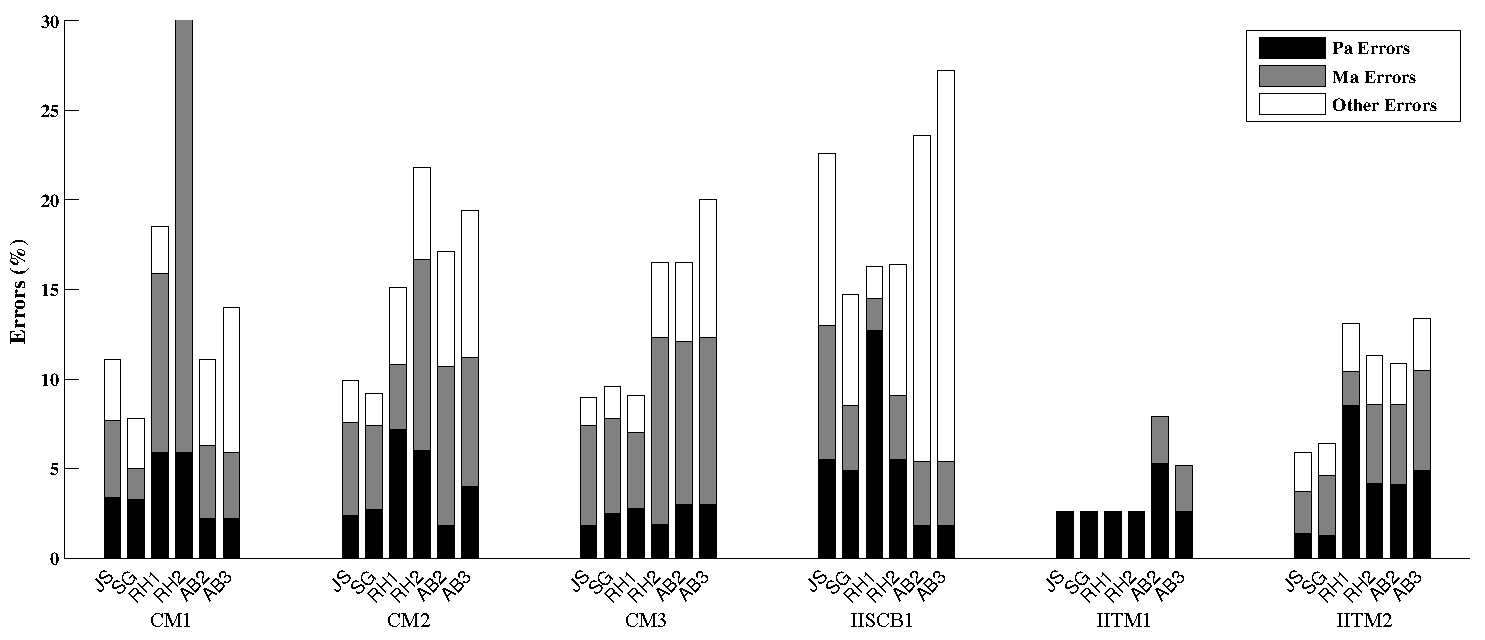
\includegraphics[width=\figSizeHundred]{ch05_preprocessing/figures/ErrorAnalysis_Without_MF.pdf}
	\end{center}
	\caption{Percentage of excerpts containing each of the three different
		categories of errors (excluding octave errors): Pa, Ma and Other, when no additional metadata is used.\TODO{Fix method and dataset names}}
	\label{fig:tonic_identification_errors_without_MF}
\end{figure}

In~\figref{fig:tonic_identification_errors_without_MF} for each dataset we present the percentage of excerpts containing each of the three categories of errors for every method (when no additional metadata is used). We see that for most datasets Pa and Ma errors constitute a large proportion of the total amount of errors made by each method. These confusions make sense from a musical perspective, since in every performance of \gls{iam} one of these two \glspl{svara} (Pa or Ma) is always present in a melody in addition to Sa (the tonic pitch-class). Furthermore, the pitch distance between Sa and Pa (fifth) is
the same as the distance between Ma and higher Sa, and the pitch distance between Sa and Ma (one fourth) is same as the distance between between Pa and higher Sa. Since most approaches are based on templates or rules that consider the pitch distance between the peaks of the feature histogram, these equivalences can
cause four types of confusions: considering a Sa-Pa pair to be Ma-Sa leading to a Pa error, considering Ma-Sa to be Sa-Pa leading to a Ma error, considering
Sa-Ma to be Pa-Sa leading to a Ma error and considering Pa-Sa to be Sa-Ma leading to a Pa error.

For the approaches based on multi-pitch analysis (\acrshort{tonicid_justin} and \acrshort{tonicid_sankalp}) we observe that the only case where we get more `Other' errors compared Pa and Ma errors is for the \acrshort{tds_iisc} dataset. Since the drone sound is very weak in the excerpts of this dataset, there are cases in which the prominent peaks of the multi-pitch histogram correspond to \glspl{svara} other than Sa, Ma and Pa (which depends on the choice of the \gls{raga}). Since these approaches assume that the multi-pitch histogram represents the \glspl{svara} of the drone instrument, the peaks of the histogram are mistakenly identified as Sa and Pa or Sa and Ma, leading to an error in identification. For these specific type of excerpts the \acrshort{tonicid_ranjani_1} method produces slightly better results, as the \gls{shadja} is not inflected (i.e. there is little pitch variation) regardless of the \gls{raga}.

In many cases we observe that the percentage of Ma errors is greater than the percentage of Pa errors. For the classification based approaches, this can be
attributed to the fact that in most excerpts the drone instrument is tuned to \textit{Pa tuning} (lower Sa, middle Sa, middle Sa, lower Pa). This creates a
bias in the training set and the rules learned by the classifier work better for Pa tuning. Ma errors are also common in \acrshort{tonicid_ranjani_2}, as the estimator looks for a Sa-Pa-higher Sa pitch relation, which would also fit a Ma-tuned performance. \acrshort{tonicid_ranjani_1} on the other hand does not search for a Sa-Pa-Sa template, resulting in a low proportion of Ma errors compared to the other methods. Finally we note that most methods do not make any Ma errors on the \acrshort{tds_iitm1} dataset. This is because the items in this dataset are full concerts, each concert consisting of several pieces. Whilst Ma may be included in the melody of some of the pieces, Pa and Sa are always present. As a result, the pitch histogram for the complete concert does not contain a prominent Ma peak, meaning that it is highly unlikely for it to be selected as the tonic.

\begin{figure}
	\begin{center}
		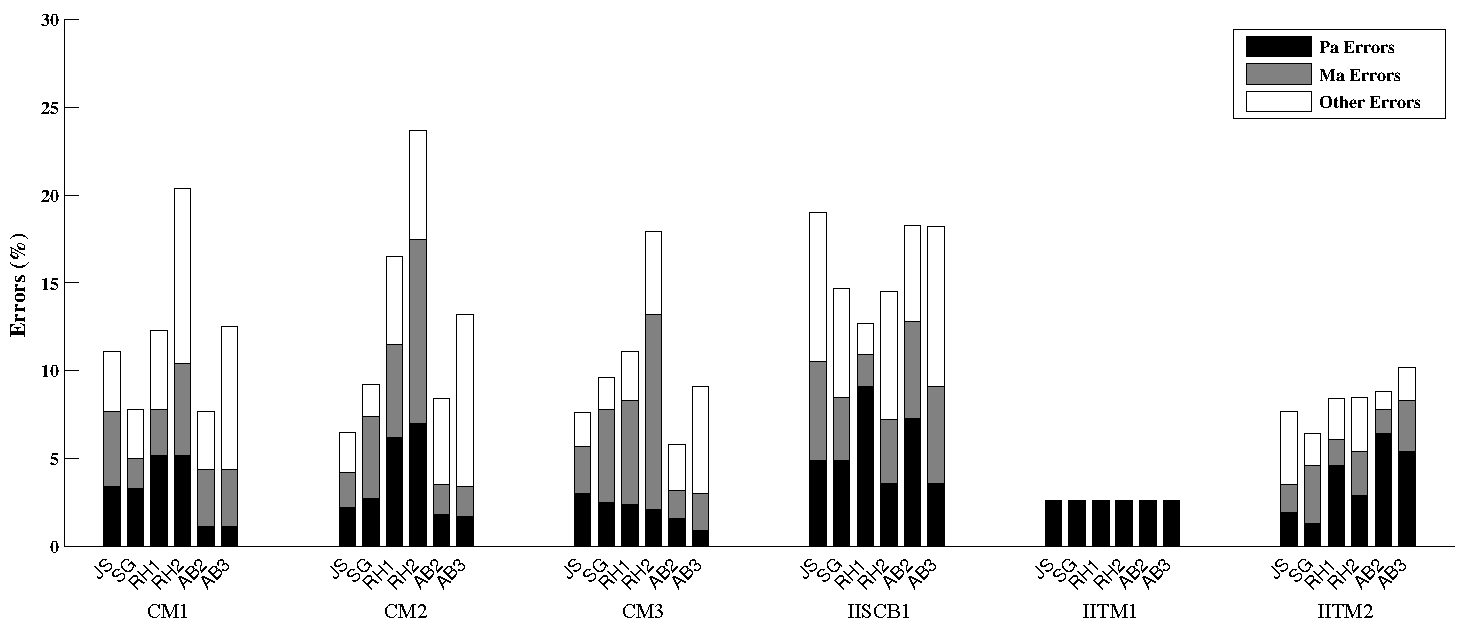
\includegraphics[width=\figSizeHundred]{ch05_preprocessing/figures/ErrorAnalysis_With_MF.pdf}
	\end{center}
	\caption{Percentage of different type of errors (Pa, Ma  and Others) by different methods on all the datasets using information regarding the gender of the singer and performance type. \TODO{Fix method and dataset names}}
	\label{fig:tonic_identification_errors_with_MF}
\end{figure}

We examine how the errors are affected once we allow methods to use gender and performance metadata, shown in ~\figref{fig:tonic_identification_errors_with_MF}. If we compare the results to those in~\figref{fig:tonic_identification_errors_without_MF}, we see
that Ma and Pa errors are reduced more than ``Other'' errors. By restricting the tonic frequency range to a single octave we prevent the
appearance of a high Sa peak, thus avoiding the possible confusion between fourths and fifths explained earlier and reducing the amount of Pa and Ma errors.

For \acrshort{tonicid_ranjani_1} and \acrshort{tonicid_ranjani_2} the percentage of Ma errors actually increases slightly after including male/female information. A large proportion of these errors were observed in excerpts with female singers. For these excerpts, the range for \gls{shadja} candidates is limited to 130-250 Hz. For this range, candidates fitting a lower Ma-middle Sa-middle Ma template would also satisfy the minimization criteria used in \acrshort{tonicid_ranjani_2}. In the case of \acrshort{tonicid_ranjani_1}, the reduced frequency range results in relatively weak peaks also being considered, and their small pitch variance can result in the wrong candidate being selected during the minimization process.

\begin{figure}
	\begin{center}
		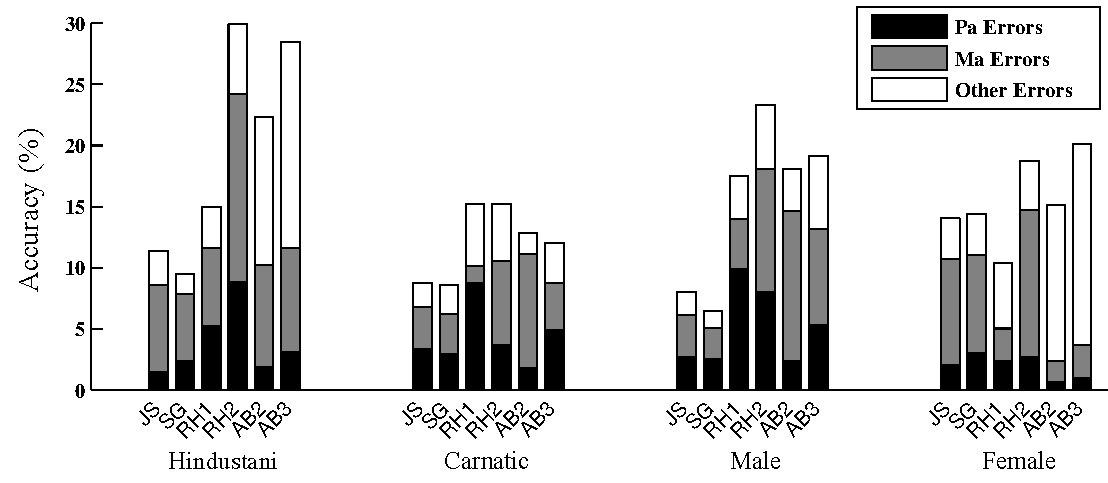
\includegraphics[width=\figSizeHundred]{ch05_preprocessing/figures/Category_Errors.pdf}
	\end{center}
	\caption{Percentage of excerpts with the different categories of errors (Pa, Ma and Others) for every method as a function of different excerpt attributes (Hindustani, Carnatic, male, female).}
	\label{fig:tonic_identification_categorywise_errors}
\end{figure}

Finally, we analyze the errors as a function of the different attributes of the excerpts (Hindustani versus Carnatic, male versus female). As in~\secref{sec:pre_processing_tonic_id_results_only_audio_data}, we use the \acrshort{tds_cm2} dataset for this analysis because it is the most balanced. Note that the methods are not provided with any metadata in addition to the audio signal. The percentage of excerpts containing each of the three categories of errors (Pa, Ma and Other) for every approach as a function of the different excerpt attributes is shown in ~\figref{fig:tonic_identification_categorywise_errors}. We see that for the classification based methods, the proportion of Ma errors is much higher in performances by female singers compared to performances by male singers. The pitch range of the tonic for female singers is such that the lower Ma resides in the frequency range where the tonic of most male singers lies. Thus, the lower Ma-middle Sa (fifth) relationship for female singers is often confused with middle Sa-Pa relationship for male singers, resulting in a high number of Ma errors. For further details and insights regarding the types of error made by the
different methods and their underlying causes we refer the reader to the publications where these methods are discussed in depth \citep{salamon2012multipitch, SGulati_MThesis2012,bellur2012knowledge,ranjani2011carnatic}.


\subsection{Summary of the Analysis }
\label{sec:pre_processing_tonic_identification_summary}

In the comparative evaluation presented above seven tonic identification methods are evaluated on six different datasets that are representative of the real-world collections of \gls{iam}. The evaluation is performed in two scenarios; first, when only audio data is input to the methods, and second, when the additional information about the gender of the singer (male or female) and  the performance type (vocal or instrumental) is given in addition to audio data. The obtained results are analyzed per dataset, and for the different characteristics of the music material. Along with the accuracies of the methods we presented an in-depth error analysis, describing different kinds of errors for different scenarios and provided plausible explanations for them.

Overall, we see that the approaches \acrshort{tonicid_justin} and \acrshort{tonicid_sankalp} that use multi-pitch based audio feature and classification methodology for selecting tonic pitch perform better than the rest. Their performance is better on all but one datasets considered in the evaluation (the exceptional dataset is small in size and contains poor quality audio recordings). In addition, the performance of these two approaches appears to be the most consistent across music traditions, gender of the singer (male or female) and type of music performance (vocal or instrumental). 

Finally, we select \acrshort{tonicid_justin} as a method to identify tonic pitch from audio recordings for all the studies conducted as a part of this dissertation. \acrshort{tonicid_justin} produces comparable results to \acrshort{tonicid_sankalp} and is relatively straightforward to implement owing to a single stage processing. Furthermore, \acrshort{tonicid_justin} does not require an estimate of predominant pitch, which is desired as it eliminates any dependence on another methods. The are two implementations of this method, which are publicly available online at \TODO{link to the code}. 


\subsection{Correcting Common Errors in Tonic Identification}
\label{sec:pre_processing_tonic_identification_correcting_errors}

As mentioned, identification of the tonic pitch of the lead artist in an audio recording is a crucial first step required for nearly all meaningful melodic analyses of \gls{iam}. Any error in the identification of tonic pitch thus propagates and has an adverse affect on the output of a melodic anlaysis task. It leads to an uncertainty whether the error is caused due to a wrong tonic pitch or because of the limitation of the melodic analysis method. Ideally, while evaluating tasks such as melodic similarity and \gls{raga} recognition we would like the tonic identification to be free from any errors. Though the accuracy obtained by the most successful tonic identification method is nearly 90\% (Table XX), even a 10\% error in tonic pitches can deteriorate the performance of these tasks. 

In this section we present an heuristic-based approach to correct frequently occurring errors in tonic identification. From table XX we see that the majority of the errors are Ma and Pa errors. We know from the musical knowledge that the tonic pitch chosen  by the performers in \gls{iam} does not change much over years and it typically remains within 2 semitones (200\,Cents). Since the accuracy of the tonic identification is nearly 90\%, for the recordings of an artist in the corpus there might only be a handful of recordings for which the tonic values are wrong. Moreover, these wrong estimates are either Ma or Pa. These errors typically correspond to a pitch value that can not be the true tonic of the singer, since it does not change a lot across recordings. Thus, such erroneous cases can be detected automatically by applying a majority voting criterion. Once detected, the wrongly estimated tonic values can be transposed to meet the most frequent tonic value of that artist in the corpus. After this step we achieve close to perfect tonic estimates for the artist. As can be imagined, this approach would work for artists that have more than 3-4 recordings in the collection, which is true for most of the artists as their recordings are ripped from their CDs.

\TODO{rephrase and make better this section.}

\section{Melody Processing}
\label{sec:data_preprocessing_melody_processing}

In this section we describe in detail all the steps applied at various stages to process melody for different melodic analyses addressed in this dissertation. These processing steps can be grouped into three main categories; predominant melody estimation (or sometimes also called as extraction), melody post-processing and melody representation. All these three steps are described at length in the subsequent sections. 

\begin{figure}
	\begin{center}
		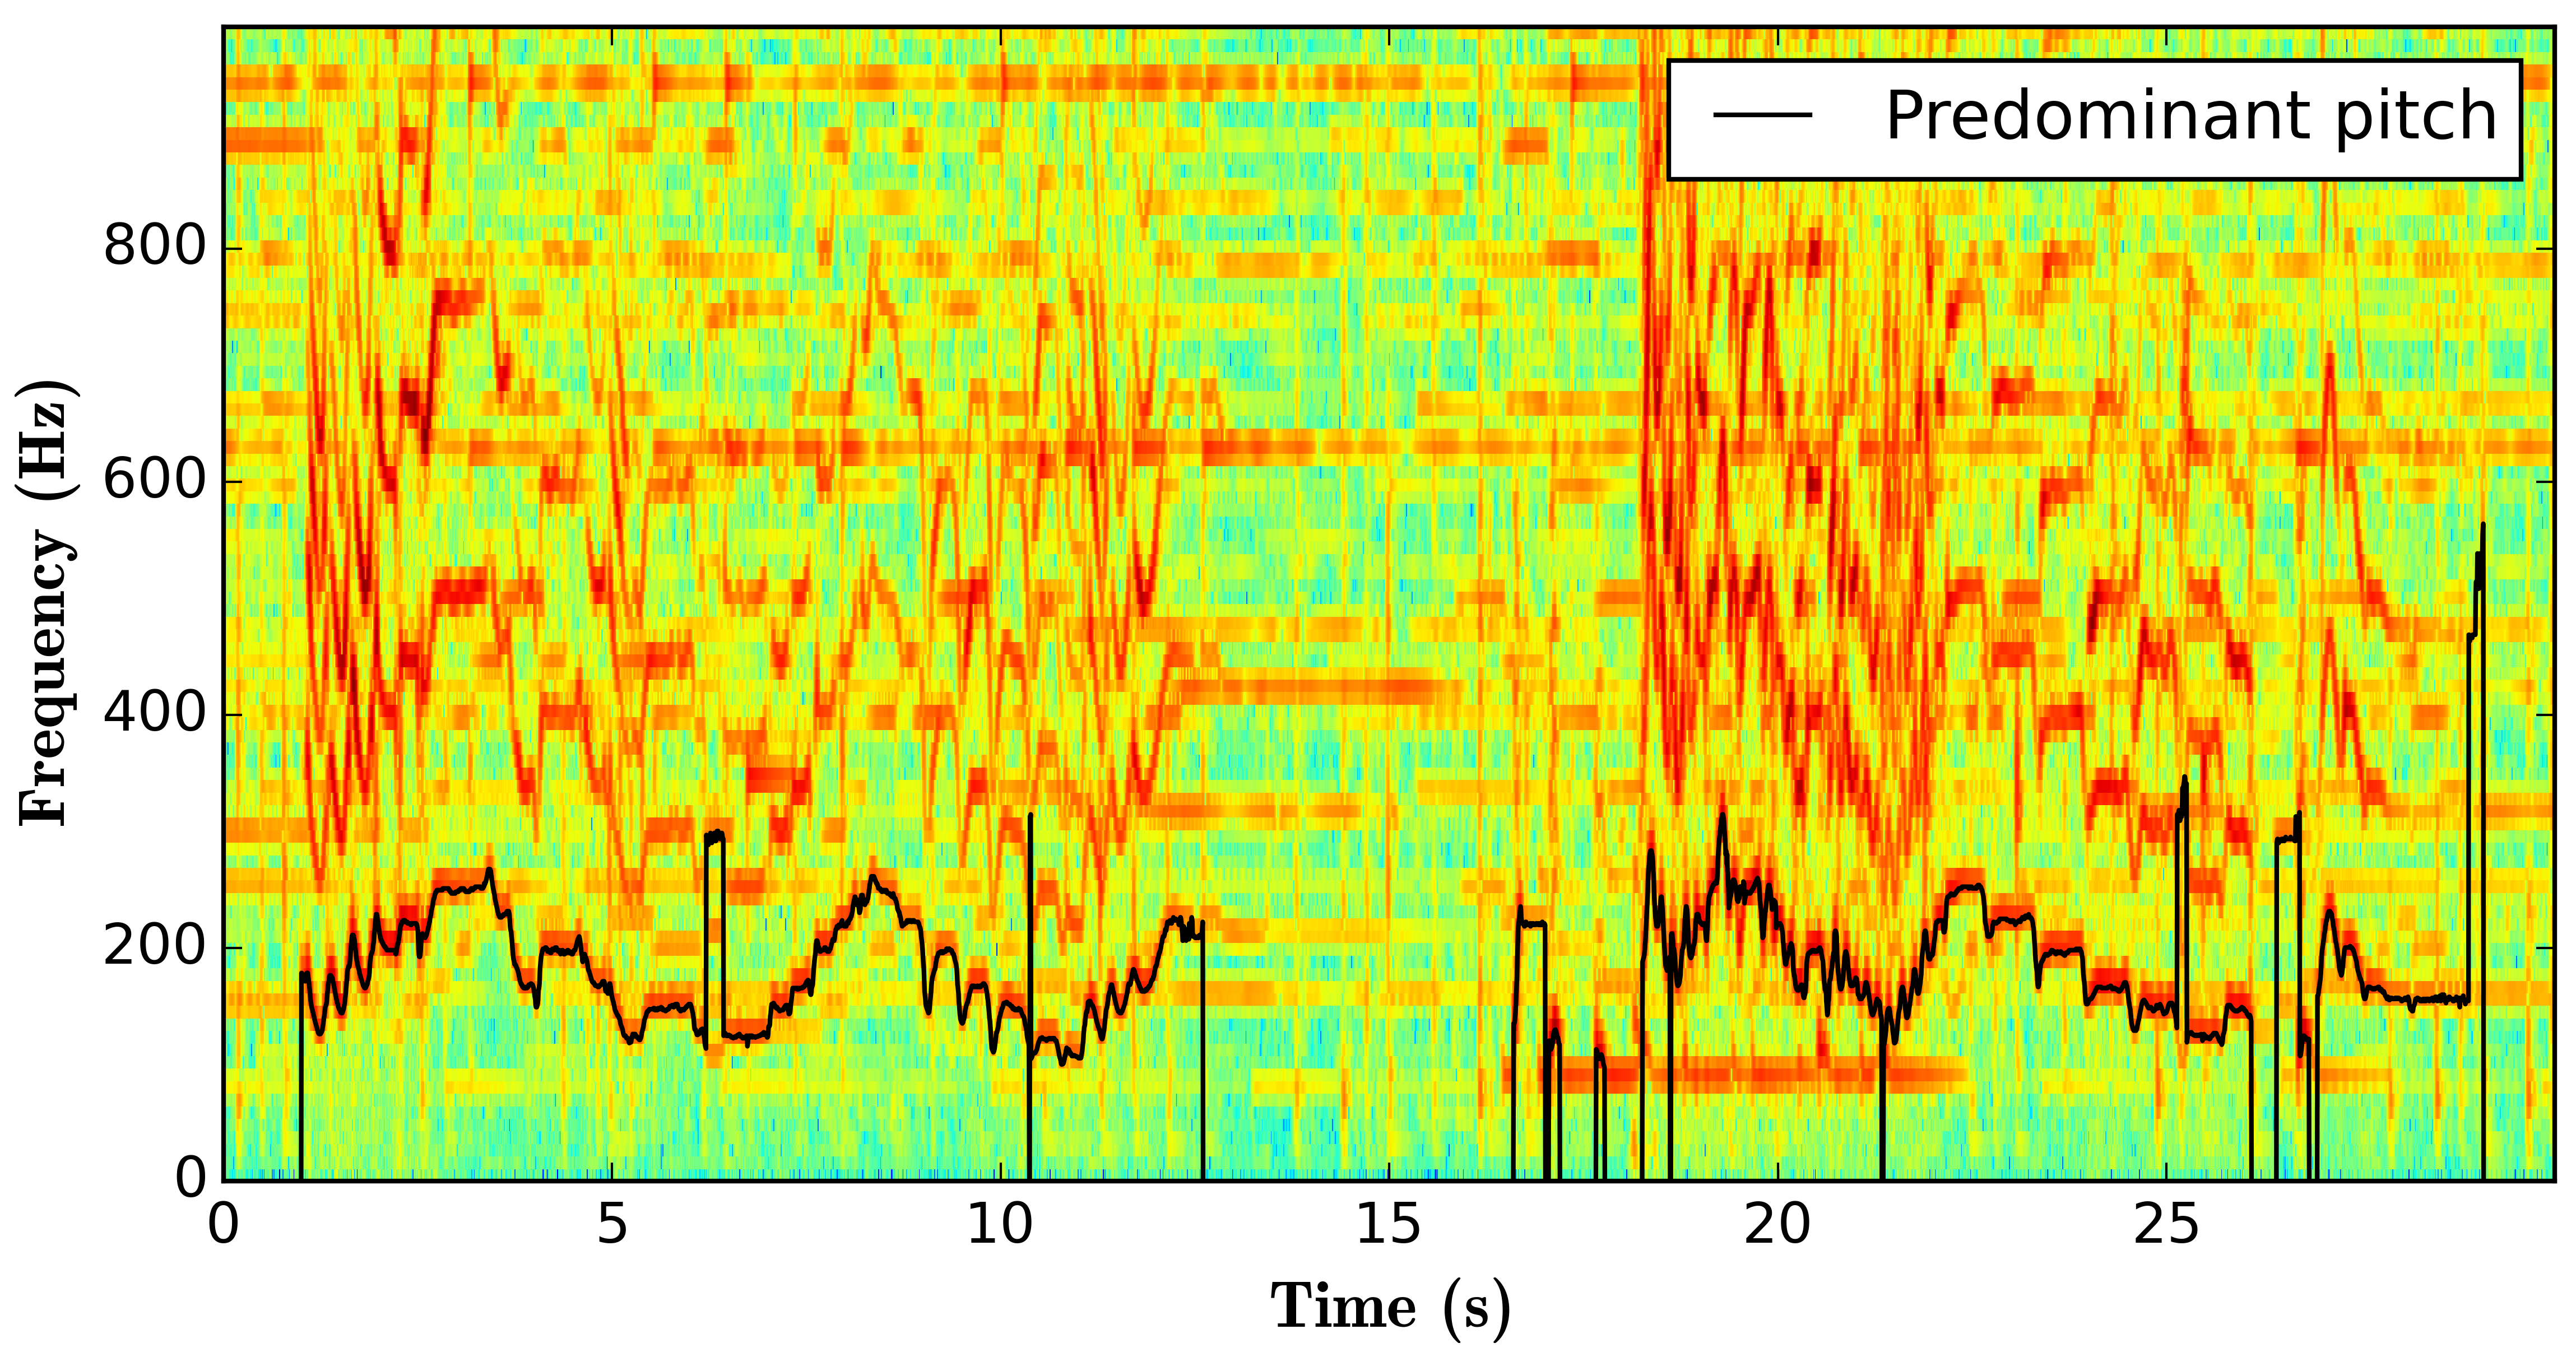
\includegraphics[width=\figSizeHundred]{ch05_preprocessing/figures/predominantMelodyExample.png}
	\end{center}
	\caption{Example of a continuous pitch contour corresponding to the predominant melodic source extracted from a polyphonic audio excerpt}
	\label{fig:predominant_melodic_fragment}
\end{figure}


\subsection{Predominant Melody Estimation}
\label{sec:data_preprocessing_predominant_melody_estimation}

The primary aim in this thesis is to develop computational models to analyze the melodic aspects of \gls{iam}. It is therefore essential to clearly understand the engineering definition of melody that we consider in this dissertation. \Gls{iam} is heterophonic in nature (Section~\TODO{XXX}), wherein there are typically two melodic lines or melodic sources; the primary source, which is the lead artist and the secondary source, which is the accompanying instrumentalist. In this dissertation we consider melody as a continuous pitch contour corresponding to the predominant melodic source (typically, the lead artist) in the audio signal. An example of a melody of an audio excerpt is shown in~\figref{fig:predominant_melodic_fragment}, where the contour represents the pitch of the lead singer at each instance in time. Usage of such a melody representation is a common practice, done by several other researchers for a variety of melody processing tasks across different music traditions~\citep{Dutta2014,Ishwar2013,Rao2014,koduri2014intonation,senturk2013score,pikrakis2012tracking}. \TODO{Add papers of other music genres for diff type of tasks} For other interesting definitions of melody we refer the readers to~\citep{Salamon2012}. 


Pitch estimation, also commonly known as pitch tracking from audio signals has been an active research topic since several decades. As indicated in Section~\TODO{XXX} the challenges in the estimation of a reliable pitch contour differ across the type of audio music signals (monophonic or polyphonic). As a result of which the performance of these algorithms vary significantly across different music genres, which also seems to be correlated with the extent of the polyphony in the music. A sparse polyphonic characteristic in audio recordings of \gls{iam} due to its heterophonic nature lessens the complexity of the task to an extent compared to the music genres such as death-metal or orchestral music. This trend is clearly visible from the past MIREX results\footnote{http://www.music-ir.org/mirex/wiki/MIREX\_HOME}. Compare the accuracy obtained by the best performing method on the \gls{iam} data set with the rest of the datasets.

In order to estimate the pitch of the predominant melodic source in the audio recordings of \gls{iam} we use Melodia algorithm, a state-of-the-art melody extraction method proposed by~\cite{Salamon2012}. This method performed favorably in MIREX~2011 (an international MIR evaluation campaign) on a variety of music genres, including \gls{iam}. This method is used in several other studies that analyze melodies extracted from audio signals~\citep{Dutta2014,Ishwar2013,Rao2014,koduri2014intonation,senturk2013score,pikrakis2012tracking}.

 %\TODO{Another motivation is that this function works on continuous contour basis, so even if the classification of contour goes wrong there is a high chance that we have obtained the contour corresponding to the violin phrase. Since that also follows the melody there are several times melodic phrases obtained in the violin voice.}

Currently, there are two implementations of Melodia algorithm available for researchers to use. We use the implementation as available in Essentia~\citep{essentia}. Essentia\footnote{https://github.com/MTG/essentia} is an open-source C++ library for audio analysis and content-based MIR. We use the default values of the parameters, except for the frame and hop sizes, which are set to 46 and 2.9\,ms, respectively. The other implementation of Melodia is available as a Vamp plugin\footnote{http://mtg.upf.edu/technologies/melodia}. 

Prior to the predominant pitch estimation we apply an equal-loudness filter available in Essentia to make the processing perceptually relevant~\TODO{ref}. For this we use the default set of parameters. Noticeably, the predominant pitch estimation algorithm also performs voicing detection. This means that the algorithm in addition to estimating the pitch also detects the time segments where the predominant voice is absent. Such time segments where the predominant melodic source is inactive are assigned a dummy pitch value (usually 0). \TODO{rephrase this part}.

For nearly all the datasets in all the tasks considered in this dissertation we use Melodia algorithm to estimate predominant pitch. There is only one exception, the \acrshort{msds_iitb_hmd} dataset, which was introduced in~\cite{Ross2012b}. This dataset is used to evaluate the task of computing melodic similarity. This dataset along with audio recordings and melodic phrase annotations includes semi-automatically extracted predominant pitch contour~(\secref{sec:corpus_melodic_similarity_dataset}). Using the pitch contours provided along with the dataset allows us to compare the output of our method with other studies. In addition, since these pitch contours are nearly free from any octave errors, we avoid propagating errors to subsequent stages, and thus, evaluate the task of melodic similarity more reliably. 

All the methods reported in this dissertation primarily utilize tonal aspects of melody. However, for some of the tasks considered in this work such as melodic similarity, usage of loudness and timbral aspects of melody might be worth exploring. These features largely capture the phonetics related aspects and might be important in studying artist specific nuances in renderings of melodic phrases. To get an idea about the type of information captured by these features and their usefulness we take an example here. We synthesize the harmonic series corresponding to a voice extracted from an excerpt of Carnatic music. During the synthesis we force the pitch of the voice to a monotone while keeping the other aspects (loudness and timbre) intact. The original excerpt\footnote{original link}, extracted predominant pitch\footnote{pitch synthesizes} and the synthesized monotone voice\footnote{monotone sunthesis} is available for listening on Freesound. In addition, we also show the spectogram of the original excerpt and the monotone synthesis in Figure~\TODO{spectrogram} After listening to this example we get an idea about the amount of useful information that is left behind if we just consider the pitch aspect of the melody in the analysis. Exploiting loudness and timbral aspects for melodic analysis is left for future work.

\TODO{Obtaining pitch tracks using Dunya? should we give that info in each feature or just at once we show it for all? Maybe the specific version that we have used can be given in specific sections}
%Thoughts
%\begin{itemize}
%	\item What did we want to extract from the audio for the purpose of this thesis work. What are the dimensions of the melody that we don't consider. 
%	\item how is that fullfilled by predominant melody
%	\item Caution to the readers about the usage of the word melody.
%	\item what do we do to extract predominant melody. This problem being simpler compared to the western popular music genres.
%	\item parameter settings
%	\item motivation to choose this algorithm
%	\item How can one use it, have we shared our melody representations?
%	\item Sampling rate depends on the task, hence we talk about that when we talk about the task
%\end{itemize}

\subsection{Pitch Post-processing}
\label{sec:data_preprocessing_pitch_postprocessing}

Predominant pitch estimation is not yet a solved problem and the output pitch contour is still far from being perfect. While these algorithms get better over years, a number of errors in predominant pitch estimation can be alleviated by post-processing the pitch contour. During post-processing we mainly try to correct the spurious pitch octave jumps and smoothen the extracted pitch contour. In addition to these two operations, for certain tasks we interpolate the unvoiced regions in the melody that correspond to the short breath pauses taken by the artists. In subsequent sections we describe these post-processing steps in detail.


\subsubsection{Correcting Spurious Pitch Jumps}
\label{sec:data_processing_correcting_pitch_jumps}

One of the most frequently occurring errors in pitch estimation is detecting pitch in the wrong octave, commonly referred to as an octave error. Identifying and correcting such an error during a post-processing step for the case of a monophonic signal (containing a single harmonic series) is fairly easy\TODO{reference}. One can compare the energy of the partials with the total energy of the audio frame to infer if the estimated pitch value corresponds to the actual fundamental frequency. However, for the case of a polyphonic signal the task becomes much more challenging. 


We alleviate this problem to an extent by restricting ourselves to a specific set of pitch octave errors occurring over short duration of time. Instead of identifying a pitch octave error for an individual audio frame, which as we mentioned is a challenging task for a polyphonic audio signal, we exploit the temporal continuity of melody to detect such errors. We explain the intuition behind our method with the help of an example shown in Figure~\TODO{fig}. The ground truth pitch contour is shown in XXX and the estimated contour in XXX. If we analyze an audio frame between time XX and XX seconds, automatically identifying if there is an pitch octave error or not is a challenging task. However, analyzing the pitch continuity we can easily detect an anomalous pitch jump at time XX seconds. This is due to the fact that in a real-world scenario such a drastic pitch jump do not occur naturally. By analyzing the amount of frequency difference across the pitch transition we can infer to an extent the type of pitch error and can subsequently correct it. In this example the frequency jump at time XX seconds is XXX cents. Knowing that there is another jump in the other direction at time XX makes it more probably that the pitch segment between time XX and XX seconds suffers from an octave error. We describe this heuristic-based approach in~\algoref{alg:algorithmPitchCorrection}. In this algorithm $\mathrm{winSize}$ is set to 1\,s and $\mathrm{silenceCentValue}$ is set to $1200*\log2(\epsilon)$, where $\epsilon$ is of the order of $10^{-17}$.

\renewcommand{\algorithmiccomment}[1]{\bgroup\hfill\tiny//~#1\egroup}

\begin{algorithm}
	\caption{Correcting spurious pitch octave jumps}
	\label{alg:algorithmPitchCorrection}
	\begin{algorithmic}  
		\State {\bf Input:} pitch sequence (p) of length N samples in Cents scale
		\State jumpType = zeros(N)	

		\For{ii=0; ii<N; ii++}							\Comment{Detecting type of pitch transition}
			\State diff = p[ii+1]-p[ii]
			\If{abs(diff)\%1200 <= 300}
				\If {diff > 0}
					\State jumpType[ii+1]=3			\Comment{Positive octave jump}
				\ElsIf {diff<0}
					\State jumpType[ii]=4			\Comment{Negative octave jump}
				\EndIf
			\ElsIf {abs(diff)>=600}
				\If {p[ii]<= silenceCentValue}
					\State jumpType[ii+1]=1			\Comment{Unvoiced to voiced}
				\ElsIf {p[ii+1]<= silenceCentValue}
					\State jumpType[ii]=2			\Comment{Voiced to unvoiced}
				\ElsIf {diff>0}
					\State jumpType[ii+1]=5			\Comment{Other positive pitch jump}
				\Else
					\State jumpType[ii]=6			\Comment{Other negative pitch jump}
				\EndIf
			\EndIf
		\EndFor

		\For {ii=0; ii<N-winSize; ii++}				\Comment{Fixing pitch octave jumps}
			\State shift = 0
			\State indJumps = where(jumpType[ii:ii+winSize]!=0)			
			\If {len(indJumps) == 2}				\Comment{Process only when two jumps are detected}
				\State i1 = indJumps[0] + ii
				\State i2 = indJumps[1]	+ ii			
				\If {jumpType[i1] + jumpType[i2] == 3}		
					\State jumpType[i1] = 0
					\State continue			\Comment{Do nothing for unvoiced to voiced to unvoiced}
				\EndIf
				
				\If {jumpType[i1]\%2 = 1 and jumpType[i2]\%2 = 0 }
					\If {jumpType[i1] == 3 and jumpType[i2] != 6}
						\State shift = 1200*round((p[i1] - p[i1-1])/1200)
					\ElsIf {jumpType[i2] == 4 and jumpType[i1] != 5}
						\State shift = 1200*round((p[i2] - p[i2+1])/1200)
					\ElsIf {jumpType[i1] == 1}
						\State shift = 100*round((p[i2] - p[i2+1])/100)
					\ElsIf {jumpType[i2] == 2}
						\State shift = 100*round((p[i1] - p[i1-1])/100)
					\EndIf
				\EndIf
			\EndIf
			\State p[i1:i2+1] = p[i1:i2+1] - shift
			\State jumpType[i1] = 0
			\State jumpType[i2] = 0		
		
		\EndFor
		
	\end{algorithmic}
\end{algorithm}


\subsubsection{Pitch smoothening}
\label{sec:data_processing_pitch_smoothening}

This processing step aims to remove the spurious pitch jumps lasting over a few frames and to smooth the pitch contours. We start by performing a median filtering over the estimated pitch contour\TODO{ref}. The window length chosen for median filtering is 50\,ms. Subsequently, to smooth the pitch contour we apply a low-pass filtering by using a Gaussian window\TODO{ref}. The window size and the standard deviation of the Gaussian window is set to 50\,ms and 10\,ms, respectively. In Figure \TODO{do the figure} we show an example of a pitch segment before and after applying median filtering and Gaussian smoothening. We see that the spurious pitch jumps are removed and the pitch contour appears smooth.


\subsubsection{Pitch Interpolation}
\label{sec:data_processing_pitch_interpolation}

In renditions of melodic phrases in \gls{iam} often there are unvoiced segments lasting over a small time interval. These unvoiced segments either correspond to short breath-pauses taken by vocalists or they correspond to the consonants in the lyrics, which are unvoiced in nature. There are several challenges in handling these unvoiced segments in the computation of melodic similarity. One of the biggest challenges is to assign a meaningful numerical value to unvoiced melodic regions such that it does not deteriorate the computation of melodic similarity. Besides, such unvoiced segments might not exist in all occurrences of a melodic phrase. Therefore, in order to avoid the complexities arising from the unvoiced melodic segments, we interpolate such segments and assign them meaningful pitch values. We perform a linear interpolation across all the unvoiced regions that last for less than 300\,ms. An example of an interpolated unvoiced segment is shown in Figure XXX. \TODO{we can show a distribution of pause durations in melodies of IAM}


\subsection{Melody Representation} 
\label{sec:pre_processing_melody_representation}


\subsubsection{Hertz to Cent Conversion}
\label{sec:data_processing_cent_conversion}

The perception of musical intervals for human beings is logarithmic in nature with respect to pitch (or fundamental frequency in Hz). Thus, in order for the pitch representation to be musically meaningful,  we convert the estimated predominant pitch values from Hertz to Cents (logarithmic scale) following the Eq XX.

\begin{equation}
\label{eq:hertz_to_cent_conversion}	
p_i = 1200~\log_2\left(\frac{f_i}{f_r}\right) ,
\end{equation}

\noindent where $f_r$ is the reference tuning frequency which typically in the case of western popular (or even classical) music is set to an integer multiple or sub-multiple of 440\,Hz. 

For the case of \gls{iam} as pointed out in \secref{sec:pre_processing_tonic_identification} there is no such standard reference frequency to which all the instruments across different performances are tuned to. Every lead artist chooses a tonic pitch using which the \gls{tanpura} and the rest of the instruments are tuned. Therefore for a meaningful comparison of melodies and melodic phrases across recordings of different artists we normalize the predominant pitch by the tonic of the lead artist. We perform this normalization by considering the reference frequency $f_r$ in \eqnref{eq:hertz_to_cent_conversion} as the tonic frequency of the lead artist estimated for every recording (\secref{sec:pre_processing_tonic_identification}).  


\subsubsection{Pitch Resampling}
\label{sec:data_processing_pitch_resampling}

An optimal sampling rate of predominant melody can be argued to depend on the particular computational task under study. For certain tasks such as analysis of melodic ornaments in \gls{iam}\TODO{refs} a high sampling rate might be desired. Whereas, for computationally complex tasks such as melodic pattern discovery and search, a sampling rate as low as possible but at the same time sufficient to capture melodic nuances might be preferred. In order to avoid predominant melody computation for different sampling rates used in different experiments, we often resample the predominant melody contours extracted once at a high sampling rate. Pitch contours are decimated to a lower sampling rate by simply downsampling them by an integer factor. The downsampling factor is decided based on the sampling rate used in a particular experiment. Since the pitch contours as mentioned above are low-pass filtered, we avoid any aliasing issues that might arise due to downsampling. 

Note that all the processing blocks listed in this section are not employed in all the experiments. The description of the methods in the subsequent chapters will contain details about the processing blocks used in the experiment. \TODO{Where can we obtain the implementation}

\section{\titlecap{\glsentrytext{nyas} \glsentrytext{svara} Segmentation}}
\label{sec:pre_processing_nyas_segmentation}

Musical melodies contain hierarchically organized events that follow a specific grammar~\citep{Patel07BOOK}. Some of these events are musically more salient than others and act as melodic landmarks. Cadential notes in classical Western music~\citep{GroveCadence} or \gls{karvai} regions in Carnatic music~\citep{sambamoorthy:1998} are examples of such landmarks. While some of these landmarks can be identified based on a fixed set of rules, others do not follow any explicit set of rules and are learned implicitly by a musician through music education and practice. A computational analysis of these landmarks can discover some of these implicitly learned rules and help in developing musically aware tools for music exploration, understanding and education. 

Occurrence of a \gls{nyas} in Hindustani music melodies is an example of such a melodic landmark that we investigate in this section. A detailed description of \gls{nyas} is provided in \secref{sec:backgroung_nyas_description}. Typically, occurrence of a \gls{nyas} delimits melodic phrases, which constitute one of the most important characteristic of a \gls{raga}. Analysis of \gls{nyas} is thus a crucial step towards melodic analysis of Hindustani music. In particular, automatically detecting occurrences of \gls{nyas} (from now on referred as \gls{nyas} segments) will aid in melody segmentation, which is a crucial step in melodic phrase discovery. However, detection of \gls{nyas} segments is a challenging computational task, as the prescriptive definition of \gls{nyas} is very broad, and there are no fixed set of explicit rules to quantify this concept~\citep[p. 73]{Dey2008}. It is through rigorous practice that a seasoned artist acquires perfection in the usage of \gls{nyas}, complying to the r\={a}g grammar and exploring creativity through improvisation at the same time. 


\begin{figure}
	\begin{center}
		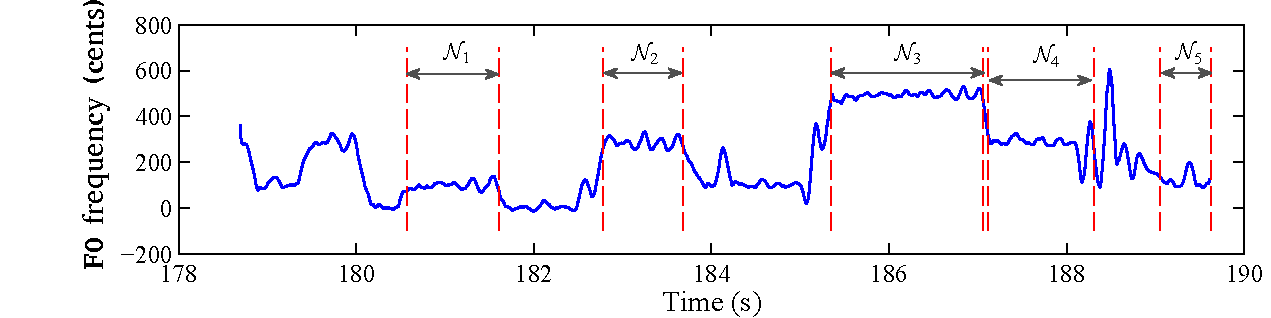
\includegraphics[width=\figSizeHundred]{ch05_preprocessing/figures/NyasFragmentChallenge.pdf}
	\end{center}
	\caption[Fragment of a pitch contour showing \gls{nyas} segments]{Fragment of a pitch contour showing \gls{nyas} segments denoted by $N_i$ ($i={1...5}$)\TODO{If time permits redo fig with diff aspect ratio}}
	\label{fig:nyas_segments_example}
\end{figure}

From a computational perspective, the detection of \gls{nyas} segments is challenging due to the variability in segment length, melodic characteristics and the different melodic contexts in which \gls{nyas} is rendered. To illustrate this point we show a fragment of pitch contour in~\figref{fig:nyas_segments_example}, annotated with \gls{nyas} segments denoted by $N_i$ ($i={1...5}$). We see that the \gls{nyas} segment length is highly varied, where $N_5$ is the smallest \gls{nyas} segment (even smaller than many non-\gls{nyas} segments) and $N_3$ is the longest \gls{nyas} segment. In addition, pitch contour characteristics also vary a lot due to the presence of \gls{alankar}\footnote{Characteristic pitch movements acting as ornaments during a \gls{svara} rendition\TODO{do we want to keep footnotes for musical concepts?}}. The pitch characteristics of a segment depends on the \gls{raga} and scale degree of the \gls{nyas}, and adds further complexity to the task~\citep{Bagchee1998}. For example, in~\figref{fig:nyas_segments_example}, $N_1$ and $N_3$ have a small pitch deviation from the mean \gls{svara} frequency, whereas, $N_2$ and $N_4$ have significant pitch deviation (close to 100\,cents in $N_5$). Large pitch deviations also pose a challenge in segmentation process. Further, melodic context such as the relative position with respect to a non-voiced or long melodically constant region plays a crucial role in determining a \gls{nyas} segment. Because of these factors the task of \gls{nyas} segment detection becomes challenging and requires sophisticated learning techniques together with musically meaningful domain specific features.

In computational analysis of \gls{iam}, \gls{nyas} segment detection has not received much attention in the past. To the best of our knowledge, only one study with the final goal of spotting melodic motifs has indirectly dealt with this task~\citep{Ross2012}. In it, the authors considered performances of a single r\={a}g and focused on a very specific \gls{nyas} \gls{svara}, corresponding to a single scale degree: the fifth with respect to the tonic, the `Pa' \gls{svara}. This \gls{svara} is considered as one of the most stable \glspl{svara}, and has minimal pitch deviations. Thus, focusing on it oversimplified the methodology developed in~\cite{Ross2012} for \gls{nyas} segment detection. \TODO{Should we move this to state of the art? + svara notation should be replaced by a glossary item?}. Note that the concept of landmark has been used elsewhere, with related but different notions and purposes. That is the case with time series similarity~\citep{Perng00ICDE}, speech recognition~\citep{Jansen08JASA,Chen12ICASSP}, or audio identification~\citep{Duong13ICASSP}.

In this section, we describe our method for detecting occurrences of \gls{nyas} \gls{svara} in Hindustani music melodies. The description is based on our work presented in~\cite{gulati2014Landmark}. The method consists of two main steps: segmentation based on domain knowledge, and segment classification based on a set of musically motivated pitch contour features. There are three main reasons for selecting this approach over a standard pattern detection technique (for example \gls{dtw}). First, the pitch contour of a \gls{nyas} segment obeys no explicit patterns, hence the contour characteristics have to be abstracted. Second, information regarding the melodic context of a segment can be easily interpreted in terms of discrete features. Third, we aim to measure the contribution of a specific feature in the overall classification accuracy (for example, if contour variance and length are the most important features for the classification). This is important in order to corroborate the results obtained from such data driven approaches to that from musicological studies. In the subsequent sections we first describe our method~(Section XX), present the methodology used for evaluation~(Section XX), discuss the results and summarize our findings~(Section XX).

\subsection{Method}
\label{sec:pre_processing_nyas_id_method}

The block diagram of the proposed method for \gls{nyas} segmentation is shown in~\figref{fig:bd_nyas_segmentation}. It consists of four main processing blocks; predominant pitch estimation and representation, segmentation, feature extraction, and segment classification and fusion. These processing blocks are described in the following sections.

\begin{figure}
	\begin{center}
		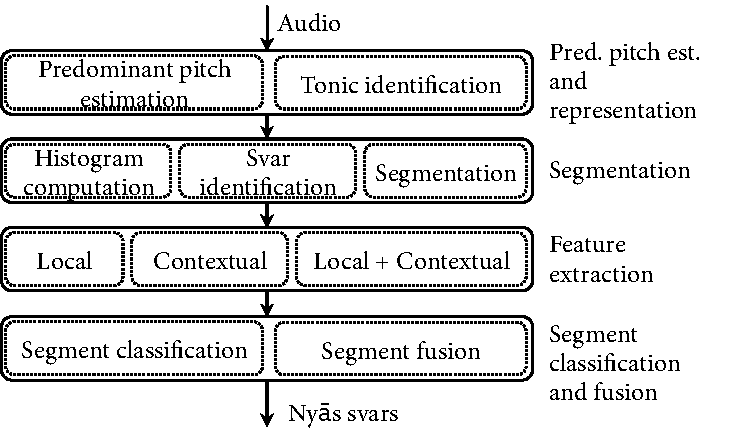
\includegraphics[width=\figSizeEightyFive]{ch05_preprocessing/figures/BlockDiagramNyasSegmentation.pdf}
	\end{center}
	\caption{Block diagram of the proposed approach for \gls{nyas} segmentation.}
	\label{fig:bd_nyas_segmentation}
\end{figure}

\subsubsection{Predominant Pitch Estimation and Representation}

For estimating pitch of the the predominant melodic source we use the procedure described in~\secref{sec:data_preprocessing_predominant_melody_estimation} with the same set of parameters. We do not perform any post-processing on the estimated pitch contours. Pitch estimated in Hertz is converted to Cent scale and is normalized by the tonic of the lead artist in the recording as described in~\secref{sec:data_processing_cent_conversion}. Tonic pitch of an audio recording is estimated using the method proposed by~\cite{salamon2012multipitch} as it was shown to be the most robust and accurate method in~\secref{sec:pre_processing_tonic_identification_summary}. 


\subsubsection{Segmentation}
\label{sec:nyas_svara_segmentation_method}

\Gls{nyas} segment is a rendition of a single \gls{svara} and the aim of the segmentation process is to detect the \gls{svara} boundaries. However, \glspl{svara} contain different \glspl{alankar} as discussed before where pitch deviation with respect to the mean \gls{svara} frequency can go roughly up to 200\,cents. This characteristic of a \gls{svara} in Hindustani music poses a challenge to segmentation. To illustrate this, in Figure~\ref{fig:nyas_segmentation_illustration} we present an example of a \gls{nyas} segment (between $T_1-T_9$, centered around mean \gls{svara} frequency $S_n=990$\,cents). The pitch deviation in this \gls{nyas} segment with respect to the mean \gls{svara} frequency reaches almost 100\,cents (between $T_5-T_6$). Note that here the reference frequency, i.e. 0\,cent correspond to the tonic pitch of the lead singer.

\begin{figure}
	\begin{center}
		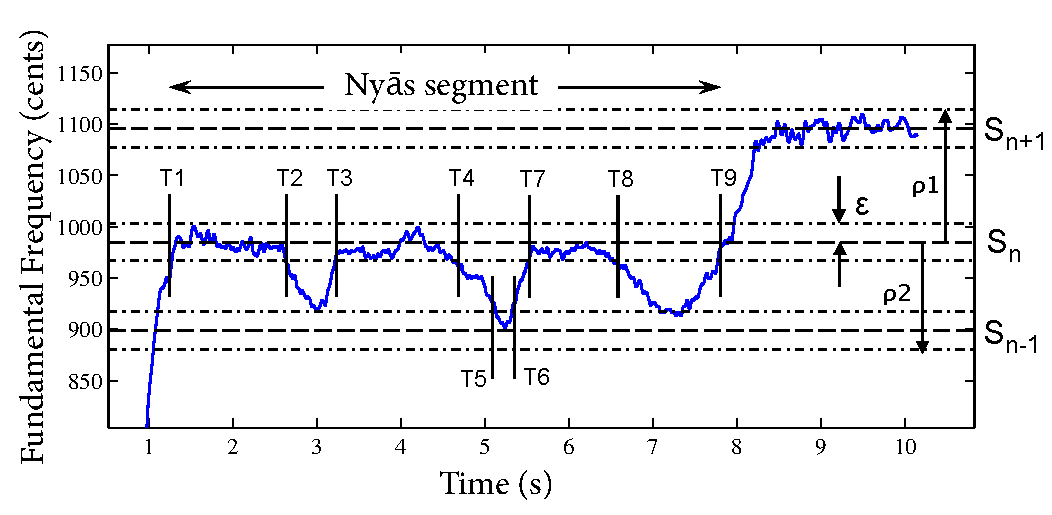
\includegraphics[width=\figSizeNinety]{ch05_preprocessing/figures/NyasSegmentationMethod.pdf}
	\end{center}
	\caption{Fragment of a pitch contour containing a \gls{nyas} segment ($T_1-T_9$), where $T_i$s denote time stamps and $S_n$s denote mean \gls{svara} frequencies. The pitch deviation within the \gls{nyas} segment ($T_1-T_9$) is almost 100\,cents ($T_5-T_6$).}
	\label{fig:nyas_segmentation_illustration}
\end{figure}

We experiment with two different methods for segmenting melodies: \gls{pls}, a classical, generic approach used for the segmentation of time series data~\citep{keogh2004segmenting}, and our proposed method, which incorporates domain knowledge to facilitate the detection of \gls{nyas} boundaries. For \gls{pls} we use a bottom-up segmentation strategy as described by~\cite{keogh2004segmenting}. Bottom-up segmentation methods involve computation of residual error incrementally for each sample of time series. When the residual error satisfies a pre-defined criterion a new segment is created. Out of the two typical criteria used for segmentation, namely average and maximum error, we choose the latter because, ideally, a new segment should be created as soon as the melody progresses from one \gls{svara} to the other. In order to select the optimal value of the allowed maximum error, which we denote by $\epsilon$, we iterated over four different values and chose the one which resulted in the best performance. Specifically, for $\epsilon=\lbrace 10, 25, 50, 75\rbrace$, $\epsilon=75$\,cents yielded the best performance. We rejected $\epsilon\geq 100$\,cents in early experimentation stages because few \glspl{svara} of a r\={a}g are separated by an interval of 100\,cents and, therefore, the segmentation output was clearly unsatisfactory.

To make the segmentation process robust to pitch deviations, we propose a method based on empirically-derived thresholds. Unlike \gls{pls}, our proposed method computes a pitch histogram and uses that to estimate mean \gls{svara} frequencies before the computation of residual error. This allows us to compute the residual error with respect to the mean \gls{svara} frequency instead of computing it with respect to the previous segment boundary, as done in \gls{pls}.  In this way our proposed method utilizes the fact that the time series being segmented is a pitch contour where the values of the time series hover around mean \gls{svara} frequencies. The mean \gls{svara} frequencies for an excerpt are estimated as the peaks of the histogram computed from the estimated pitch values. An octave folded pitch histogram is computed using a 10\,cent resolution and subsequently smoothened using a Gaussian window with a variance of 15\,cents. Only the peaks of the normalized pitch histogram which have at least one peak-to-valley ratio greater than 0.01 are considered as \gls{svara} locations. As peaks and valleys we simply take all local maximas and minimas over the whole histogram. In~\figref{fig:pitch_histogram_nyas_segmentation} we show an example of an octave folded normalized  pitch histogram used for estimating mean \gls{svara} frequencies. The estimated mean \gls{svara} frequencies are indicated by circles. We notice that the pitch values corresponding to a \gls{svara} span a frequency region and not a single value.


\begin{figure}
	\begin{center}
		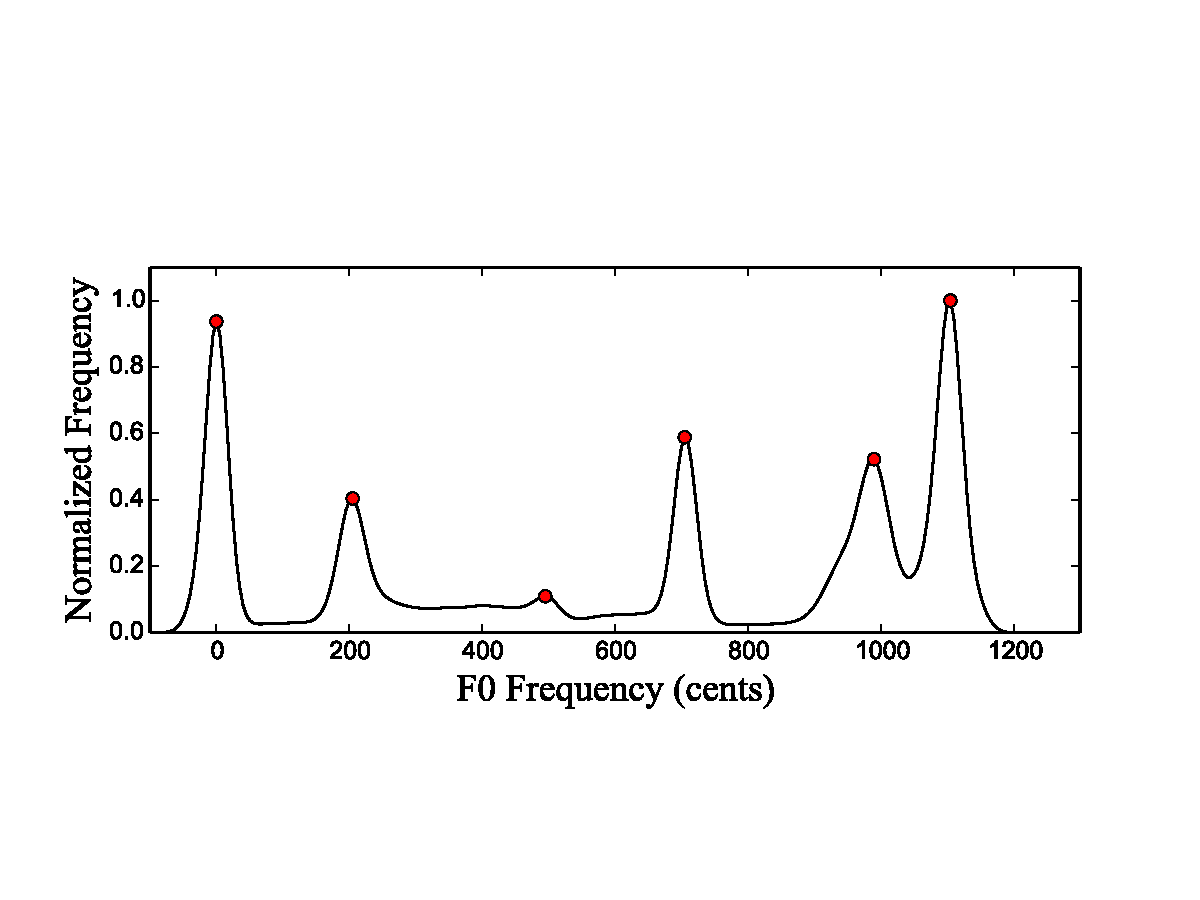
\includegraphics[width=\figSizeNinety]{ch05_preprocessing/figures/swarOnHistogramForNyasSegmentation.pdf}
	\end{center}
	\caption{Normalized octave folded pitch histogram used for estimating mean \gls{svara} frequencies. Estimated mean \gls{svara} frequencies are indicated by circles.}
	\label{fig:pitch_histogram_nyas_segmentation}
\end{figure}

After we estimate mean frequencies of all the \glspl{svara} in a piece, we proceed with their refinement. For the $n$-th \gls{svara} $S_n$, we search for contiguous segments within a deviation of $\varepsilon$ from $S_n$, that is, $\vert S_n-P_i \vert < \varepsilon$, for~$i\in[1,N]$, where $P_i$ is the fundamental frequency value (in cents) of the $i$-th sample of a segment of length $N$. In Figure~\ref{fig:nyas_segmentation_illustration}, this corresponds to segments $[T_1,T_2]$, $[T_3,T_4]$, and $[T_7,T_8]$.

Next, we concatenate two segments $[T_a,T_b]$ and $[T_e,T_f]$ if two conditions are met:
\begin{enumerate}
	\item $P_i-S_n < \rho_1$ and $S_n-P_i < \rho_2$, for $i\in[T_b,T_e]$, where $\rho_1 = S_{n+1}-S_n + \varepsilon$ and $\rho_2 = S_n-S_{n-1} + \varepsilon$. 
	\item $T_c-T_d < \delta$, where $\delta$ is a temporal threshold and $[T_c,T_d]$ is a segment between $T_b, T_e$ such that $\vert S_m-P_i\vert <\varepsilon$ for $i\in[T_c,T_d]$ for $m\in [S_{n-1}, S_{n+1}]$ and $m \neq n$.
\end{enumerate}

In simple terms, we concatenate two segments if the fundamental frequency values between them do not deviate a lot (less than $\rho_1$ and $\rho_2$) and the time duration of the melody in close vicinity (less than $\epsilon$) of neighboring \glspl{svara} is not too large (less than $\delta$). We repeat this process for all \gls{svara} locations. In our experiments, we use $\varepsilon = 25$\,cents and $\delta=50$\,ms, which were empirically obtained. In the example of~\figref{fig:nyas_segmentation_illustration}, we see that the two conditions apply for segments $[T_1,T_2]$ and $[T_3,T_4]$, and not for $[T_3,T_4]$ and $[T_7,T_8]$ because $T_6-T5>\delta$. Notice that we can already derive a simple binary flatness measure $\nu$ for $[T_a, T_b]$, $\nu=1$ if $\vert S_n-P_i \vert< \epsilon$ for $i \in [T_a, T_b]$ for any $n$ and $\nu=0$ otherwise. 

\subsubsection{Feature Extraction}
\label{sec:pro_processing_nyas_segmentation_feature_extraction}

We extract musically motivated melodic features for segment classification, which resulted out of discussions with musicians. For every segment obtained following the process mentioned above, three sets of melodic features are computed: local features~(L), which capture the pitch contour characteristics of the segment, contextual features~(C), which capture the melodic context of the segment, and a third set combining both of them~(L+C) in order to analyze if they complement each other. Initially, we considered 9 local features and 24 contextual features:

\begin{description}
	\item[Local Features:] segment length, mean and variance of the pitch values in a segment, mean and variance of the differences in adjacent peak locations of the pitch sequence in a segment, mean and variance of the  peak amplitudes of the pitch sequence in a segment, temporal centroid of the pitch sequence in a segment normalized by its length, and the above-mentioned flatness measure $\nu$ (we use the average segmentation error for the case of \gls{pls}).
	\item[Contextual Features:] segment length normalized by the length of the longest segment within the same breath phrase\footnote{Melody segment between consecutive breaths of a singer. We consider every unvoiced segment (i.e.,~a value of 0 in the pitch sequence) greater than 100\,ms as breath pause.}, segment length normalized by the length of the breath phrase, length normalized with the length of the previous segment, length normalized by the length of the following segment, duration between the ending of the segment and succeeding silence, duration between the starting of the segment and preceding silence, and all the local features of the adjacent segments.
\end{description}

However, after preliminary analysis, we reduced these features to 3 local features and 15 contextual features. As local features we selected length, variance, and flatness measure ($\nu$). As contextual features we selected all of them except the local features of the posterior segment. This feature selection was done manually, performing different preliminary experiments with a subset of the data, using different combinations of features and selecting the ones that yielded the best accuracies.

\subsubsection{Classification and Segment Fusion}

Each segment obtained in~\secref{sec:nyas_svara_segmentation_method} is classified into \gls{nyas} or non-\gls{nyas} based on the extracted features described in~\secref{sec:pro_processing_nyas_segmentation_feature_extraction}. To demonstrate that the predictive power of the considered features is generic and independent of a particular classification scheme, we employ five different algorithms exploiting diverse classification strategies~\citep{Hastie09BOOK}: trees (Tree), \gls{knn}, \gls{nb}, \gls{lr}, and \gls{svm} with a radial basis function kernel. We use the implementations available in scikit-learn~\citep{scikitlearn}, version 0.14.1. We use the default set of parameters with few exceptions in order to avoid over-fitting and to compensate for the uneven number of instances per class. Specifically, we set \texttt{min\_samples\_split=10} for Tree, \texttt{fit\_prior=False} for \gls{nb}, \texttt{n\_neighbors=5} for \gls{knn}, and for \gls{lr} and \gls{svm} \texttt{class\_weight=`auto'}.

For out-of-sample testing we implement a cross-fold validation procedure. We split the data set into folds that contain an equal number of \gls{nyas} segments, the minimum number of \gls{nyas} segments in a musical excerpt. Furthermore, we make sure that no instance from the same artist and \gls{raga} is used for training and testing in the same fold.

After classification, boundaries of \gls{nyas} and non-\gls{nyas} segments are obtained by merging all the consecutive segments with the same segment label. During this step, the segments corresponding to the silence regions in the melody, which were removed during classification, are regarded as non-\gls{nyas} segments.

\subsection{Experimental Setup}
\label{sec:pre_processing_nyas_segmentation_experimental_setup}

\subsubsection{Music Collection and Annotations}

For evaluation of this task we use the \gls{nyas} dataset \acrshort{nds_cm} as described in~\secref{sec:corpus_nyas_dataset}. As explained, this dataset contains both commercially released polyphonic music recordings and in-house monophonic recordings. As melodic characteristics of a \gls{nyas} segment might depend on the artist and the chosen \gls{raga}, the dataset includes performances by 8 artists in 16 different \glspl{raga} to ensure diversity and representativeness.

\subsubsection{Evaluation Measures and Statistical Significance}

We evaluate two tasks, \gls{nyas} segment boundary annotation, and \gls{nyas} and non-\gls{nyas} segment label annotation. For the evaluation of \gls{nyas} boundary annotations we use hit rates as in a typical music structure boundary detection task~\citep{Ong05ICMC}. While calculating hit rate, segment boundaries are considered as correct if they fall within a certain threshold of a boundary in the ground-truth annotation. Using matched hits, we compute standard precision, recall, and F-score for every fold and average them over the whole data set. The choice of a threshold however depends on the specific application. Due to the lack of scientific studies on the just noticeable differences of \gls{nyas} \gls{svara} boundaries, we computed results using an arbitrary selected threshold of 100\,ms. Label annotations are evaluated using standard pairwise frame clustering method as described in~\cite{levy2008structural}. Frames with same duration as threshold value for the boundary evaluation (i.e. 100~ms) are considered while computing precision, recall, and F-score. 

For assessing statistical significance we use the Mann-Whitney U test~\citep{mann1947test} with $p<0.05$ and assuming an asymptotic normal distribution of the evaluation measures. To compensate for multiple comparisons we apply the Holm-Bonferroni method~\citep{holm1979simple}, a powerful method that also controls the so-called family-wise error rate. Thus, we end up using a much more stringent criteria than $p<0.05$ for measuring statistical significance.

\subsubsection{Baselines}

Apart from reporting the accuracies for the proposed method and its variants, we compare against some baseline approaches. In particular, we consider \gls{dtw} together with a \gls{knn} classifier ($K=5$). For every segment, we compute its distance from all other segments and assign a label to it based on the labels of its $K$ nearest neighbors, using majority voting. As the proposed method also exploits contextual information, in order to make the comparison more meaningful, we consider the adjacent segments in the distance computation with linearly interpolated values in the region corresponding to the segment. For comparing with the variant of the proposed method that uses a combination of the local and contextual features, we consider adjacent segments together with the actual segment in the distance computation. As this approach does not consider any features, it will help us in estimating the benefits of extracting musically-relevant features from \gls{nyas} segments. 

In addition, to quantify the limitations of the adopted evaluation measures, we compute a few random baselines. The first one (RB1) is calculated by randomly planting boundaries (starting at 0\,s) according to the distribution of inter boundary intervals obtained using the ground-truth annotations. For each segment we assign the labels `\gls{nyas}' with a a priory probability (same for all excerpts) computed using ground truth annotations of the whole data set. The second one (RB2) is calculated by planting boundaries (starting at 0\,s) at even intervals of 100\,ms and assigning class labels as in RB1. Finally, the third one (RB3) considers the exact ground-truth boundaries and assigns the class labels randomly as in RB1 and RB2. Thus, with RB3 we can directly assess the impact of the considered classification algorithms. We found that RB2 achieves the best accuracy and therefore, for all the following comparisons we only consider RB2.

%\begin{table} 
%\centering
%\begin{tabular}{ c | c c c }
%\hline\hline
%  		&	RB1	&	RB2	&	RB3\\
%\hline
% 	\gls{nyas} Boundary		&  0.10 & 0.17 &1.0  \\ 
%%\hline 	
%	\gls{nyas} Region		& 0.56 & 0.69 & 0.64 \\
%\hline\hline
%\end{tabular}
%
%\caption{F-scores for \gls{nyas} boundary estimation and \gls{nyas} region
%estimation using random baseline methods. \XXX{J}{S}{Why not adding a row or column in the general results tables??}}
%	\label{tab:randombaseline}
%\end{table}

\subsection{Results and Discussion}
\label{sec:preprocessing_nyas_segmentation_results_and_discussion}

We evaluate two tasks, \gls{nyas} segment boundary annotation, and \gls{nyas} and non-\gls{nyas} segment label annotation. For both the tasks, we report results obtained using two different segmentation methods (\gls{pls} and the proposed segmentation method), five classifiers (Tree, \gls{knn}, \gls{nb}, \gls{lr}, \gls{svm}), and three set of features (local (L), contextual(C) and local together with contextual (L+C)). In addition, we report results obtained using a baseline method (DTW) and a random baseline (RB2).

In Table~\ref{tab:nyas_segmentation_boundary_accuracy} we show the results of \gls{nyas} boundary annotations. First, we see that every variant performs significantly better than the best random baseline. RB2 yields an F-score of 0.184 while the worst variant tested reaches 0.248. Next, we see that the proposed method achieves a notably higher accuracy compared to the DTW baseline. Such difference is found to be statistically significant, with the only exception of the NB classifier. For a given feature set, the performance differences across classifiers are not statistically significant. The only exceptions are Tree and NB, which yield relatively poor and inconsistent performances over different feature sets. We opted to not consider these two classifiers in the following comparisons. Among  feature sets, the performance differences are not statistically significant between \gls{pls} variants (Table~\ref{tab:nyas_segmentation_boundary_accuracy}, top rows), whereas for the case of the proposed segmentation method (Table~\ref{tab:nyas_segmentation_boundary_accuracy}, bottom rows), we find that the local features perform significantly better than the contextual features and their combination does not yield consistent improvements. Finally, we see that the best results are obtained using the proposed segmentation method together with the local features, with a statistically significant difference to its competitors. Furthermore, the worst accuracy obtained using the proposed segmentation method is notably higher than the best accuracy using \gls{pls} method, again with a statistically significant difference.

\begin{table} 
\renewcommand{\arraystretch}{1.25}
\setlength{\tabcolsep}{6pt}
	\begin{centering}
	\begin{tabular}{ c : c : c : c c c c c c }
\tabletop
		& Feat.		&	\gls{dtw} & Tree	 &	\gls{knn} 	&	\gls{nb}		& \gls{lr} 	&	\gls{svm}\\
\tablemid
		\multirow{3}{*}{A} & 	L		&  0.356 & 0.407 & 0.447 & 0.248 & 0.449 & 0.453\\ 
		%\hline 	
		&	C		& 0.284 & 0.394 & 0.387 & 0.383 & 0.389 & 0.406 \\
		%\hline	
		&	L+C		& 0.289 & 0.414 & 0.426 & 0.409 &0.432 & 0.437 \\
\tablemid
		\multirow{3}{*}{B} &	L		& \textbf{0.524} & 0.672 & \textbf{0.719} & 0.491 & \textbf{0.736} & \textbf{0.749}\\ 
		%\hline 	
		&	C		& 0.436 & 0.629 & 0.615 & \textbf{0.641} & 0.621 & 0.673 \\
		%\hline	
		&	L+C		& 0.446 & \textbf{0.682} & 0.708 & 0.591 & 0.725 & 0.735\\  		
\tablebot		
	\end{tabular}	
	\caption[F-scores for \gls{nyas} boundary detection task]{F-scores for \gls{nyas} boundary detection using \gls{pls} method (A) and the proposed segmentation method (B). Results are shown for different classifiers (Tree, \gls{knn}, \gls{nb}, \gls{lr}, \gls{svm}) and local (L), contextual (C) and local together with contextual (L+C) features. \gls{dtw} is the baseline method used for comparison. F-score for the random baseline obtained using RB2 is 0.184.}
	\label{tab:nyas_segmentation_boundary_accuracy}
	\par	\end{centering}
\end{table}


In~\tabref{tab:nyas_segmentation_label_accuracies} we show the results for \gls{nyas} and non-\gls{nyas} label annotations. Basically, we can draw similar conclusions as with Table~\ref{tab:nyas_segmentation_label_accuracies}: (1) all method variants perform significantly better than the random baselines, (2) all the proposed method variants yield significant accuracy increments over the \GLS{dtw} baseline, and (3) no statistically significant differences between classifiers (with the aforementioned exceptions). In label annotations, unlike the boundary annotations, we find that though the local features perform better than the contextual features, the differences are not statistically significant for all the proposed method variants. Furthermore, we also see that the proposed segmentation method consistently performs  better than \gls{pls}. However, the differences are not always statistically significant.

In addition, we also investigate per-class accuracies for label annotations. We find that the performance for \gls{nyas} segments is considerably better than non-\gls{nyas} segments. This could be attributed to the fact that even though the segment classification accuracy is balanced across classes, the differences in segment length of \gls{nyas} and non-\gls{nyas} segments (\gls{nyas} segments being considerably longer than non-\gls{nyas} segments) can result in more number of matched pairs for \gls{nyas} segments.

\begin{table} 
\renewcommand{\arraystretch}{1.25}
\setlength{\tabcolsep}{6pt}
\begin{centering}	
	\begin{tabular}{ c : c : c : c  c  c  c  c  c }
\tabletop
		& Feat.	&	DTW & Tree	 &	KNN 	&	NB		& LR 	&	SVM	\\
\tablemid		
		\multirow{3}{*}{A} &   L		& \textbf{0.553} & 0.685 & 0.723 & 0.621 & 0.727 & 0.722	\\
		%\hline         
		&	C   		& 0.251 & 0.639 & 0.631  & 0.690 & 0.688 & 0.674	\\
		%\hline 
		& 	L+C		& 0.389 & 0.694 & 0.693 & 0.708 & 0.722 & 0.706	\\	
		\hline
		\multirow{3}{*}{B} & 	L		& 0.546 & \textbf{0.708} & \textbf{0.754} & 0.714 & \textbf{0.749} & \textbf{0.758} \\
		%\hdashline 	
		& 	C		&0.281 & 0.671 & 0.611 & 0.697 & 0.689 & 0.697\\
		%\hline	
		& 	L+C		& 0.332 & 0.672 & 0.710 & \textbf{0.730} & 0.743 & 0.731\\
\tablebot
	\end{tabular}
	\caption{F-scores for \gls{nyas} and non-\gls{nyas} label annotations task using \gls{pls} method (A) and the proposed segmentation method (B). Results are shown for different classifiers (Tree, KNN, NB, LR, SVM) and local (L), contextual (C) and local together with contextual (L+C) features. DTW is the baseline method used for comparison. The best random baseline F-score is  0.153 obtained using RB2. } 
	\label{tab:nyas_segmentation_label_accuracies}
\par \end{centering}
\end{table}


In general, we see that the proposed segmentation method improves the performance over \gls{pls} method in both tasks, wherein the differences are statistically significant in the former case. Furthermore, the local feature set, when combined with the proposed segmentation method, yields the best accuracies. We also find that the contextual features do not complement the local features to further improve the performance. However, interestingly, they perform reasonably good considering that they only use contextual information.


\subsection{Summary}
\label{ConclusionAndFutureWork}

We described a method for detecting \gls{nyas} segments in melodies of Hindustani music. We divided the task into two broad steps: melody segmentation and segment classification. For melody segmentation we proposed a method which incorporates domain knowledge to facilitate \gls{nyas} boundary annotations. We evaluated three feature sets: local, contextual and the combination of both. We showed that the performance of the proposed method is significantly better compared to a baseline method using standard \gls{dtw} based distance and a $K$ nearest neighbor classifier. Furthermore, we showed that the proposed segmentation method outperforms a standard approach based on \gls{pls}. A feature set that includes only the local features was found to perform best. However, we showed that using just the contextual information we could also achieve a reasonable accuracy. This indicates that \gls{nyas} segments have a defined melodic context which can be learned automatically. \TODO{Where can we obtain the implementation from? and the experiment scripts?}


\section{Tani Segmentation}
\label{sec:pre_processing_tani_segmentation}

A concert of Carnatic music typically contains a solo percussion section towards the end of the concert, referred to as \gls{tani} avartanam or \gls{tani} in short. The duration of such segments typically varies from 2 to 25\,min depending on the artist and the context. The main percussion instrument in Carnatic music is \gls{mridangam}, which becomes the lead instrument during this section. Along with the \gls{mridangam} there are other percussion instruments often played in \gls{tani} section such as \gls{kanjira} and \gls{ghatam}. Though \gls{mridangam} is a percussion instrument and is basically a kind of a barrel drum, its sound has tonal characteristics. Like other accompanying instruments in Carnatic music such as \gls{tanpura} and violin, \Gls{mridangam} is also tuned at the tonic of the lead artist. Due to the tonal acoustical characteristics of \gls{mridangam} sound, and because of the long duration of \gls{tani} sections, the pitch estimation algorithm detects and tracks pitch contours during \gls{tani} sections instead of detecting these sections as non-voiced segments. Notice that the \gls{mridangam} strokes during short (lasting over roughly 1-20 seconds) unvoiced segments such as breath-pauses are correctly detected as non-voiced by the predominant pitch estimation algorithm. This is due to the fact that during such sections predominant pitch corresponds to voice, which has significantly high energy compared to the background percussion signal. 


\begin{figure}
	\begin{center}
		
\includegraphics[width=\figSizeNinety]{ch05_preprocessing/figures/figure_todo.pdf}
	\end{center}
	\caption{Discovered pair of patterns in predominant pitch contours corresponding to \gls{mridangam} strokes in a \gls{tani} section.}
	\label{fig:pitch_pattern_tani}
\end{figure}

Failing to detect \gls{tani} sections as non-voiced segments and tracking pitch corresponding to \gls{mridangam} strokes poses a challenge in the discovery of melodic patterns. Percussion patterns and rhythm cycles often contain recurring stroke patterns, and therefore, pitch fragments from \gls{tani} section are frequently discovered as highly similar patterns. An example of a discovered pair of pitch patterns that correspond to \gls{mridangam} strokes is shown in~\figref{fig:pitch_pattern_tani}. We see that the patterns are close to exact repetitions. Since we aim to discover patterns in melodies of \gls{iam} (\chapref{chap:melodic_pattern_processing}), patterns discovered from \gls{tani} sections are undesired. There can be two approaches to avoid such unwanted patterns in the final output; 1) post-process the discovered pitch patterns and detect if they belong correspond to \gls{mridangam} strokes, 2) discard pitch contours corresponding to \gls{tani} section in the pre-processing step. We follow the second approach and discard segments of the pitch contours that correspond to \gls{tani} sections from the input given to the pattern discovery method. Discarding such segments upfront has several advantages. First, detection of \gls{tani} sections in audio recording appears to be an easier task compared to characterizing pitch contours as belonging to melody or \gls{mridangam} strokes. This is mainly because of the considerable amount of timbral differences across the sections where melody (typically voice) is present and where it is not (\gls{tani} sections). Also, such computational tasks of classifying an audio segment based on its timbral characteristics is well studied in \gls{mir}\TODO{ref}. In~\figref{fig:spectrogram_of_tani_segment} we show the waveform and the spectrogram of a voice segment and a \gls{tani} section to demonstrate the timbral differences between the two. Another reason for choosing the latter approach is because discarding \gls{tani} sections upfront reduces the computational complexity of the pattern discovery task as these sections may typically last up to 2-25\,minutes. We therefore detect \gls{tani} sections in the audio recordings and discard the pitch segments corresponding to these sections in the pre-processing step.

\begin{figure}
	\begin{center}
		
\includegraphics[width=\figSizeNinety]{ch05_preprocessing/figures/figure_todo.pdf}
	\end{center}
	\caption{Waveform and spectrogram of a voice and a \gls{tani} section in an audio recording of Carnatic music.}
	\label{fig:spectrogram_of_tani_segment}
\end{figure}

We detect \gls{tani} segments in audio recordings using a classification-based approach \TODO{ref}. To feed the classifiers we extracted 13~MFCC coefficients, spectral centroid, spectral flatness and pitch salience \citep{slaney1998auditory} from the audio signal using Essentia~\citep{essentia}. We iterated over 23, 46 and 92\,ms frame sizes and chose the one which resulted in a better classification accuracy. We set the hop size as half the frame size and all other parameters to their default values. Next, we computed means and variances of these features over 2\,s non-overlapping segments (also sometimes referred to as texture window). For training, we used a labeled audio music dataset containing 1.5~hours of mixed voice and violin recordings and 1.5~hours of solo percussion recordings. To assess the performance of the extracted features, we performed a leave-one-out cross-validation. We experimented with five different algorithms exploiting diverse classification strategies~\cite{Hastie09BOOK}: decision trees (Tree), \glsreset{knn}, \glsreset{nb}, \glsreset{lr}, and \glsreset{svm} with a radial basis function kernel. We use the implementations of the classifiers as available in scikit-learn version~0.14.1~\citep{scikitlearn}. We used the default set of parameters with few exceptions to avoid over-fitting and to compensate for the uneven number of instances per class. We set \texttt{min\_} \texttt{samples\_split=10} for Tree, \texttt{fit\_prior=False} for \gls{nb}, \texttt{n\_neighbors=5} for \gls{knn}, and for \gls{lr} and \gls{svm} \texttt{class\_weight=`auto'}. 

The combination of the frame size of 46\,ms and the \gls{svm} classifier yielded the best performance (96\% accuracy), with no statistically significant difference to the performance with the Tree (95.5\%) and the \gls{knn} (95\%), for the same frame size. We finally chose \gls{knn} because of its low complexity. The accuracy of detecting a \gls{tani} section can be improved further by a simple post-processing step. Since \gls{tani} is a single continuous segment in an audio recording, the class labels of the texture windows predicted by the classifier can be median filtered to remove the spurious labels lasting over a few frames. This ensures a continuity in labels across texture windows and avoids short non-voiced regions during the main performance (not the \gls{tani} section) being classified as \gls{tani} segments.  \TODO{Rephrase this tani segmentation section}

\TODO{Implementation of method and dataset?}

\section{Summary}
\label{sec:preprocessing_summary}

We here summarize what we described in this chapter. Basically repetition of stuff. Do we really need this?\textsl{}
